\clearpage\section{Recovered historical local polyphase manuscript}\label{app:recovered}
This is the complete substantive body of the reconstructed Annals textual
copy, preserved to retain its derivations and original parameter ranges.
The recovered text is not certified as the exact original TeX bytes. Its
historical theorem headings distinguish these statements from the current
numbered core. Preservation is not a blanket proof audit or Lean certificate:
in particular the broader Amice analytic pullback and depleted branches,
finite-field modal minimality and unrestricted infinite polyphase claims
retain their historical evidence scope. The current formal statement map
records only the individually identified interfaces in the main text.

All 14 original figure files were absent from the recovered source. This
reading edition supplies new reconstructions at their retained labels and
captions. These are explanatory schematics and exact finite examples, not
recovered original artwork. The reproducible program
\nolinkurl{tools/reconstructed_figures.py} checks the displayed finite data.
The modulo-seven inverse plot uses the corrected positive tail
$6,5,2,6,5,2,\ldots$. A reconstructed illustration does not upgrade the
historical proof or formalization status. The historical bibliography file is also absent. Its citation keys
are preserved in the bibliography as unresolved source records, without
invented bibliographic entries. Superseded claims about the divisor-branch
finite-difference problem have local notices directing the reader to the
current theorem. The remaining higher kernel-valuation and unrestricted
local-to-global questions remain open in their stated scopes.

\subsection{Introduction}\label{hist:sec:introduction}

Euler numbers carry several kinds of local information at once. Their indices have residue addresses. Their coefficient transforms have triangular depth. Their local expansions have Mahler degree. Their congruences depend on the valuation of the transfer kernel and on the valuation of the source value in the row being reconstructed. These pieces should not be merged into one undifferentiated congruence calculation.

This article begins with the Hurwitz product
\[
(a\starh b)_n
=
\sum_{r=0}^{n}
\binom nr a_rb_{n-r}.
\]
Over a field of characteristic zero it is multiplication of exponential generating functions. Over a finite field it realizes the additive group algebra through the exponential modes \(\epsilon_u=(u^n)_{n\geq0}\). This finite algebra gives an exact proof of the standard window period. Hurwitz series rings are treated in \cite{Keigher1997,BarberoCerrutiMurru2018}. The finite difference and umbral background may be found in \cite{Roman1984,Comtet1974,GrahamKnuthPatashnik1994}.

Fix an odd prime \(p\), a divisor \(m\mid p-1\), and put
\[
h=\frac{p-1}{m}.
\]
The reduced standard window inverse is defined by
\[
\sum_{q=0}^{n}
\binom{mn}{mq}e_q^{(m,p)}
=
\delta_{n0}
\quad\text{in }\FF_p.
\]
We prove that
\[
e_{n+h}^{(m,p)}=e_n^{(m,p)}
\qquad(n\geq1).
\]
The result first follows from subgroup symmetry in the finite Hurwitz algebra. A second proof shows that the standard window operator preserves the finite space of sequences that are \(h\) periodic after their constant term. The two arguments expose different parts of the same finite character structure.

The central change in this edition is the treatment of the odd and dyadic Euler formulas. They are no longer presented as unrelated reconstruction devices. For each prime \(p\) we define an even source series \(H_p\) and an inverse kernel \(K_p\) satisfying
\[
K_p(t)H_p(t)=\operatorname{sech}t.
\]
At an odd prime,
\[
H_p(t)=\cosh^2(pt)\operatorname{sech}t,
\qquad
K_p(t)=\operatorname{sech}^2(pt).
\]
At the dyadic prime,
\[
H_2(t)=\frac{\sinh(2t)\sinh t}{2t^2},
\qquad
K_2(t)=\frac{4t^2}{\sinh^2(2t)}.
\]
The coefficient convolution is identical in form, but the kernels have different integral weights. This is the correct sense in which the local theories unify.

The dyadic kernel is substantially sharper than the separate coefficient bound alone suggests. If
\[
\frac{z^2}{\sinh^2z}
=
\sum_{r\geq0}\beta_rz^{2r}
\]
and
\[
\kappa_{2,r}=\beta_r2^{2r}(2r)!,
\]
then
\[
\vTwo(\kappa_{2,r})=4r-1
\qquad(r\geq1).
\]
Consequently, truncation after depth \(M\) is uniformly valid modulo
\[
2^{4M+3},
\]
and this exponent is optimal. The rowwise estimate records the additional binary carries in the binomial coefficient. Classical congruence theory for Euler families is extensive \cite{CarlitzLevine1960,Young1999,Young2001,Sun2008,Chen2004}. The formulas here are stated as exact coordinate identities. Historical priority requires a separate theorem by theorem comparison.

The second expansion concerns local interpolation. The exponent of the finite unit group moves every unit mode into a principal unit neighborhood. Binomial expansion then gives a Mahler series whose depth \(r\) coefficient gains at least \(Lr\) digits when the chosen jump is the identity modulo \(p^L\). The same argument applies to polynomial exponential modes and to invertible matrix state systems. Mahler interpolation and the Amice transform are classical \cite{Mahler1958,Amice1964,Robert2000}. The local unit structure and valuation tools used here are standard \cite{Koblitz1984,Serre1979,Washington1997,Gouvea1997}.

The odd Euler source contains one nonunit base. Removing that base gives an analytic unit source and an interpolation of a depleted Euler sequence on every even character branch. The dyadic source is already analytic on \(\Zp\) after a removable singularity is filled. It yields a direct analytic interpolation of \(E_{2n}\) on \(\mathbb Z_2\). These branches are then refined by the substitution
\[
x=Mq+s.
\]
The induced Mahler coefficient transform is finite and explicit. Its kernels compose exactly. At prime power radix they become sparse modulo the residue prime. Every monotone valuation ladder survives the refinement.

The remaining sections treat arithmetic lift obstructions, recurrence packets, and Chinese remainder reconstruction. The lifting obstruction is the residual defect modulo the image of the declared correction map. A recurrence packet is governed by a jump matrix \(C^N\). If one integral recurrence is fixed, all of its local realizations have one common source. These statements do not prove that arbitrary unrelated local objects have a global origin.

\begin{figure}[t]
\centering
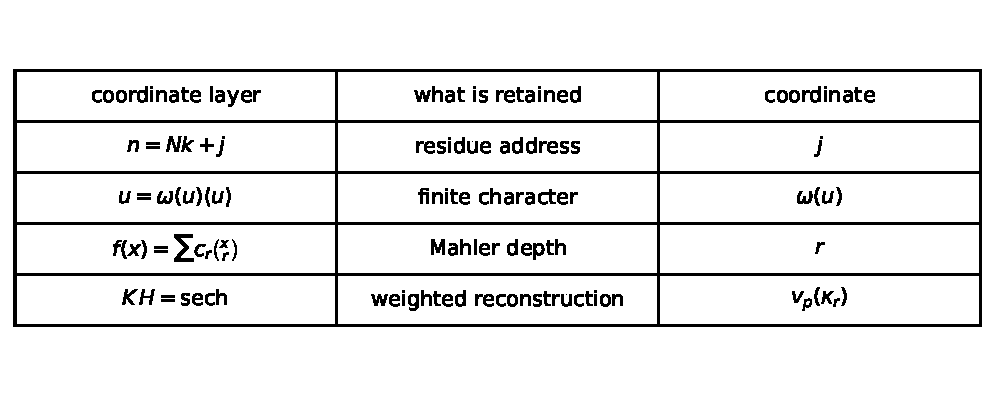
\includegraphics[width=.95\linewidth,height=3.15in,keepaspectratio]{../../figures/reconstructed/architecture.pdf}
\caption{New reconstruction. The arithmetic coordinate chain. Residue address, local character, Mahler depth, transfer weight, and reconstruction are recorded separately.}
\label{hist:fig:architecture}
\end{figure}

Four boundaries remain explicit. A period modulo \(p\) does not by itself lift to all powers of \(p\). The full finite difference estimate for every congruential reciprocal packet still requires control of the triangular inverse. Exact higher valuations of the affine polyphase kernel are not yet known in general. Chinese remainder reconstruction and finite adelic synchronization do not prove a global source for arbitrary local systems.
\subsection{Hurwitz series and finite field subgroup inversion}\label{hist:sec:hurwitz}
\par\smallskip\noindent\textbf{Current status.} This dated statement is superseded for the stated divisor-branch family by Theorem~\ref{thm:arith-divisor-base}, with the $j!$ normalization and factorial valuation loss explicitly retained. It makes no claim for unrestricted families.\par

\subsubsection{The Hurwitz ring}

\begin{histdefinition}[Hurwitz series ring]\label{hist:def:hurwitz_ring}
Let \(R\) be a commutative ring with identity. The Hurwitz series ring \(\Hcal(R)\) is the set \(R^{\NN}\) with componentwise addition and product
\[
(a\starh b)_n
=
\sum_{r=0}^{n}
\binom nr a_r b_{n-r}.
\]
Its identity is
\[
\delta=(1,0,0,\ldots).
\]
\end{histdefinition}

When the factorials are invertible, the sequence \(a\) may be written as the exponential generating series
\[
A(t)=\sum_{n\geq0}a_n\frac{t^n}{n!},
\]
and the Hurwitz product becomes ordinary multiplication. The sequence definition remains valid in every characteristic.

\begin{histdefinition}[Exponential mode]\label{hist:def:exponential_mode}
For \(u\in R\), define
\[
\epsilon_u=(u^n)_{n\geq0},
\]
where \(0^0=1\).
\end{histdefinition}

\begin{histproposition}[Addition law for modes]\label{hist:prop:mode_addition}
For every \(u,v\in R\),
\[
\boxed{
\epsilon_u\starh\epsilon_v
=
\epsilon_{u+v}.
}
\]
\end{histproposition}

\begin{proof}
The \(n\)th coefficient is
\[
\sum_{r=0}^{n}
\binom nr u^rv^{n-r}
=
(u+v)^n
\]
by the binomial theorem.
\end{proof}

\subsubsection{The finite additive group algebra}

Let \(p\) be prime. Write \(\FF_p^+\) for the additive group of the finite field.

\begin{histtheorem}[Finite field mode algebra]\label{hist:thm:mode_group_algebra}
The map
\[
\Theta:
\FF_p[\FF_p^+]
\longrightarrow
\Hcal(\FF_p),
\qquad
[u]\longmapsto\epsilon_u,
\]
is an injective algebra homomorphism. Its image is the \(p\) dimensional subalgebra spanned by the modes \(\epsilon_u\).
\end{histtheorem}

\begin{proof}
The product law follows from \cref{hist:prop:mode_addition}. To prove injectivity, suppose
\[
\sum_{u\in\FF_p}c_u\epsilon_u=0.
\]
Looking at the coordinates \(n=0,1,\ldots,p-1\) gives a Vandermonde system with matrix
\[
(u^n)_{0\leq n\leq p-1,\ u\in\FF_p}.
\]
Its determinant is the product of all differences between distinct field elements, so it is nonzero. Hence every \(c_u\) vanishes.
\end{proof}

\begin{histproposition}[Augmentation criterion]\label{hist:prop:augmentation_criterion}
Let
\[
x=\sum_{u\in\FF_p}c_u[u]
\in
\FF_p[\FF_p^+].
\]
Then \(x\) is a unit if and only if
\[
\operatorname{aug}(x)
=
\sum_uc_u
\]
is nonzero. If \(J\) is the augmentation ideal, then
\[
J^p=0.
\]
\end{histproposition}

\begin{proof}
Choose a generator \(g\) of the cyclic additive group. Then
\[
\FF_p[\FF_p^+]
\cong
\FF_p[y]/(y^p-1)
=
\FF_p[y]/(y-1)^p.
\]
The augmentation ideal is generated by \(y-1\), so its \(p\)th power is zero. Every element has the form \(a+n\) with \(a\in\FF_p\) and \(n\in J\). It is invertible exactly when \(a\neq0\), which is the augmentation condition.
\end{proof}

\begin{histcorollary}[Finite inverse formula]\label{hist:cor:finite_inverse_formula}
If \(x\) has augmentation one and \(n=x-1\), then
\[
\boxed{
x^{-1}
=
\sum_{r=0}^{p-1}(-n)^r.
}
\]
\end{histcorollary}

\begin{proof}
By \cref{hist:prop:augmentation_criterion}, \(n^p=0\). The finite geometric sum gives the inverse.
\end{proof}

\subsubsection{Subgroup selectors}

Fix a divisor \(m\) of \(p-1\). Let
\[
H_m
=
\{\zeta\in\FF_p^\times:\zeta^m=1\}.
\]
This group has order \(m\).

\begin{histdefinition}[Multiple selector]\label{hist:def:multiple_selector}
Define \(a^{(m)}\in\Hcal(\FF_p)\) by
\[
a_n^{(m)}
=
\begin{cases}
1,&m\mid n,\\
0,&m\nmid n.
\end{cases}
\]
\end{histdefinition}

\begin{histlemma}[Subgroup average]\label{hist:lem:subgroup_average}
The multiple selector has the mode expansion
\[
\boxed{
a^{(m)}
=
\frac1m
\sum_{\zeta\in H_m}
\epsilon_\zeta.
}
\]
\end{histlemma}

\begin{proof}
The \(n\)th coefficient on the right is
\[
\frac1m
\sum_{\zeta\in H_m}\zeta^n.
\]
The character sum is one when \(m\mid n\) and zero otherwise.
\end{proof}

\begin{figure}[t]
\centering
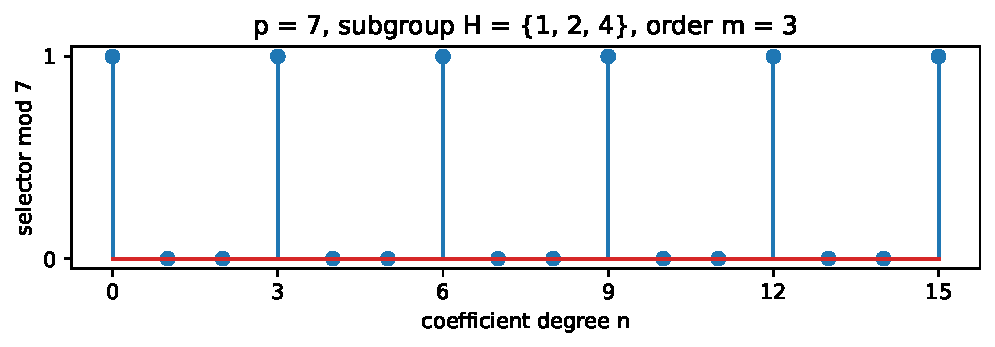
\includegraphics[width=.95\linewidth,height=3.15in,keepaspectratio]{../../figures/reconstructed/subgroup_average.pdf}
\caption{New reconstruction. A subgroup average in the additive group algebra. The highlighted modes select coefficient degrees divisible by the subgroup order.}
\label{hist:fig:subgroup_average}
\end{figure}

Since the subgroup average has augmentation one, it has a unique Hurwitz inverse. Write
\[
b^{(m,p)}
=
(a^{(m)})^{-1}.
\]

\begin{histtheorem}[Support and positive degree period]\label{hist:thm:support_period}
The inverse \(b^{(m,p)}\) has the following properties.
\begin{enumerate}
\item \(b_n^{(m,p)}=0\) unless \(m\mid n\).
\item For every positive \(n\),
\[
\boxed{
b_{n+p-1}^{(m,p)}
=
b_n^{(m,p)}.
}
\]
\end{enumerate}
\end{histtheorem}

\begin{proof}
Multiplication by an element \(\eta\in H_m\) gives an automorphism of the additive group and therefore an automorphism
\[
\epsilon_u\longmapsto\epsilon_{\eta u}
\]
of the mode algebra. The selector \(a^{(m)}\) is fixed by every such automorphism, so its unique inverse is fixed as well.

Write
\[
b^{(m,p)}
=
\sum_{u\in\FF_p}c_u\epsilon_u.
\]
Invariance gives \(c_{\eta u}=c_u\). After the change of variable \(u\mapsto\eta u\),
\[
b_n^{(m,p)}
=
\eta^n b_n^{(m,p)}
\]
for every \(\eta\in H_m\). If \(m\nmid n\), some \(\eta\) satisfies \(\eta^n\neq1\), so the coefficient vanishes.

For positive \(n\), the zero mode contributes nothing. Every nonzero mode satisfies \(u^{p-1}=1\). Hence
\[
b_{n+p-1}^{(m,p)}
=
\sum_{u\neq0}c_uu^{n+p-1}
=
\sum_{u\neq0}c_uu^n
=
b_n^{(m,p)}.
\]
\end{proof}

\begin{histdefinition}[Compressed inverse]\label{hist:def:compressed_inverse}
Set
\[
e_n^{(m,p)}
=
b_{mn}^{(m,p)}.
\]
\end{histdefinition}

\begin{histproposition}[Compressed inverse recurrence]\label{hist:prop:compressed_inverse_recurrence}
The compressed coefficients satisfy
\[
\boxed{
\sum_{q=0}^{n}
\binom{mn}{mq}
e_q^{(m,p)}
=
\delta_{n0}.
}
\]
In particular, \(e_0^{(m,p)}=1\), and the positive coefficients are determined recursively because the diagonal is one.
\end{histproposition}

\begin{proof}
Evaluate the Hurwitz identity
\[
a^{(m)}\starh b^{(m,p)}=\delta
\]
at degree \(mn\). Both factors vanish outside degrees divisible by \(m\). Reindexing the surviving terms gives the displayed recurrence.
\end{proof}

\begin{histcorollary}[Uniform compressed period]\label{hist:cor:compressed_period}
Let
\[
h=\frac{p-1}{m}.
\]
Then
\[
\boxed{
e_{n+h}^{(m,p)}
=
e_n^{(m,p)}
\qquad(n\geq1).
}
\]
\end{histcorollary}

\begin{proof}
Since \(m(n+h)=mn+p-1\), the conclusion follows from \cref{hist:thm:support_period}.
\end{proof}

\begin{histcorollary}[Rational ordinary generating function]\label{hist:cor:periodic_ogf}
In \(\FF_p[[z]]\),
\[
\boxed{
\sum_{n\geq0}e_n^{(m,p)}z^n
=
1+
\frac{
\sum_{r=1}^{h}e_r^{(m,p)}z^r
}{1-z^h}.
}
\]
\end{histcorollary}

\begin{proof}
Separate the constant coefficient and group the positive indices into residue classes modulo \(h\).
\end{proof}

\begin{histtheorem}[Exponential form and minimal period]\label{hist:thm:minimal_period}
Let
\[
G_m=(\FF_p^\times)^m.
\]
This cyclic group has order \(h\). There are uniquely determined coefficients \(d_v\in\FF_p\), indexed by \(v\in G_m\), such that
\[
\boxed{
e_n^{(m,p)}
=
\sum_{v\in G_m}d_vv^n
\qquad(n\geq1).
}
\]
The minimal positive period is the least common multiple of the orders of those \(v\) for which \(d_v\neq0\). In particular, it divides \(h\).
\end{histtheorem}

\begin{proof}
The coefficients \(c_u\) in the proof of \cref{hist:thm:support_period} are constant on the cosets of \(H_m\). For \(u\neq0\), the value \(u^m\) depends only on the coset, and every element of \(G_m\) arises. Grouping the modes by cosets gives the displayed expansion.

Distinct elements of \(G_m\) define linearly independent functions on one full period, by the Vandermonde determinant. Therefore a positive integer \(r\) is a period exactly when \(v^r=1\) for every active mode. The least such \(r\) is the stated least common multiple.
\end{proof}

\begin{histexample}[A compressed inverse modulo seven]\label{hist:ex:compressed_mod_seven}
\par\noindent\textbf{Editorial numerical correction.} The positive-index standard-window tail printed below is erroneous. The defining recurrence gives $e_1=-1\equiv6$, $e_2=5$ and $e_3=-61\equiv2\pmod7$, so the correct positive tail is $6,5,2,6,5,2,\ldots$. The period-three conclusion remains correct. The original line is retained only as a corrected historical record.\par\medskip
Take \(p=7\) and \(m=2\), so \(h=3\). The recurrence gives
\[
e_n^{(2,7)}
=
1,6,4,1,6,4,\ldots
\qquad(n\geq1).
\]
The positive tail has exact period three.
\end{histexample}

\begin{figure}[t]
\centering
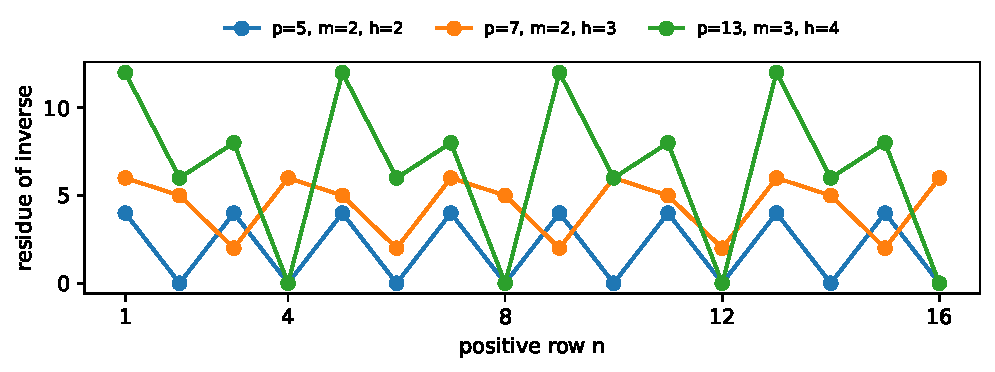
\includegraphics[width=.95\linewidth,height=3.15in,keepaspectratio]{../../figures/reconstructed/standard_periods.pdf}
\caption{New reconstruction. Several compressed inverses. Every row is periodic after the constant term, as proved in \cref{hist:cor:compressed_period}.}
\label{hist:fig:standard_periods}
\end{figure}


\subsection{Unit triangular coefficient transport}\label{hist:sec:triangular_transport}

The examples later in the paper use different kernels, but their coefficient algebra has one common form. This section records that form once. Let \(R\) be a commutative algebra over \(\QQ\), and take all coefficients in \(R\).

Let
\[
H(t)=\sum_{r\geq0}h_r\frac{t^r}{r!},
\qquad
h_0=1.
\]
There is a unique inverse
\[
K(t)=H(t)^{-1}
=\sum_{r\geq0}k_r\frac{t^r}{r!}.
\]

\begin{histtheorem}[Exact coefficient transport]\label{hist:thm:exact_coefficient_transport}
Let
\[
A(t)=\sum_{n\geq0}A_n\frac{t^n}{n!},
\qquad
S(t)=H(t)A(t).
\]
Then
\[
\boxed{
S_n
=
\sum_{r=0}^{n}
\binom nr h_rA_{n-r}.
}
\]
The inverse coordinate formula is
\[
\boxed{
A_n
=
\sum_{r=0}^{n}
\binom nr k_rS_{n-r}.
}
\]
Both transforms are lower triangular with diagonal one.
\end{histtheorem}

\begin{proof}
The first identity is the coefficient rule for the product of exponential generating functions. Multiply by \(K(t)\) and use \(K(t)H(t)=1\) for the inverse identity. The diagonal coefficient in each transform is the constant coefficient of its kernel, which is one.
\end{proof}

\begin{histcorollary}[Composition of coefficient transports]\label{hist:cor:transport_composition}
If \(U_H\) and \(U_G\) are the triangular transforms associated with unit kernels \(H\) and \(G\), then
\[
\boxed{
U_HU_G=U_{HG}.
}
\]
In particular, the inverse of \(U_H\) is \(U_{H^{-1}}\).
\end{histcorollary}

\begin{proof}
Multiplication by \(G\), followed by multiplication by \(H\), is multiplication by \(HG\).
\end{proof}

\begin{histtheorem}[Filtered triangular reconstruction]\label{hist:thm:filtered_triangular_reconstruction}
Let \(p\) be prime. Suppose
\[
A_n
=
\sum_{r=0}^{n}
\binom nr
c_rp^{w(r)}S_{n-r},
\]
where \(c_r\in\Zp\), \(S_n\in\Zp\), and
\[
w(r)\in\NN.
\]
For every precision \(L\geq1\),
\[
\boxed{
A_n
\equiv
\sum_{\substack{0\leq r\leq n\\w(r)<L}}
\binom nr
c_rp^{w(r)}S_{n-r}
\pmod {p^L}.
}
\]
When the omitted set is nonempty, the tail has valuation at least
\[
\boxed{
\min_{\substack{0\leq r\leq n\\w(r)\geq L}}
\left(
w(r)+\vp\binom nr+\vp(S_{n-r})
\right).
}
\]
\end{histtheorem}

\begin{proof}
Every omitted summand belongs to \(p^L\Zp\). The sharper statement follows by taking the minimum of the exact lower bounds for the summands and applying the nonarchimedean triangle inequality.
\end{proof}

\begin{histremark}\label{hist:rem:triangular_freedom}
An arbitrary invertible triangular matrix can encode an arbitrary sequence. The transforms retained here have an explicit generating kernel and a visible filtration. Those two features make exact inversion and uniform truncation possible.
\end{histremark}

\subsection{Congruential reciprocal packets}\label{hist:sec:congruential}

\subsubsection{Residue sections of the exponential series}

For integers \(N\geq1\) and \(0\leq j<N\), define
\[
\Ecal_{N,j}(t)
=
\sum_{n\geq0}
\frac{t^{Nn+j}}{(Nn+j)!}.
\]
The forced factor \(t^j\) may be removed without changing the residue address.

\begin{histdefinition}[Congruential reciprocal packet]\label{hist:def:congruential_packet}
Define
\[
\boxed{
\Ccal_{N,j}(t)
=
\frac{t^j/j!}{\Ecal_{N,j}(t)}
=
\sum_{n\geq0}
C_{N,j}(n)
\frac{t^{Nn}}{(Nn)!}.
}
\]
\end{histdefinition}

\begin{histtheorem}[Triangular inverse system]\label{hist:thm:triangular_inverse}
The coefficients satisfy \(C_{N,j}(0)=1\) and
\[
\boxed{
\sum_{q=0}^{n}
\binom{Nn+j}{Nq}
C_{N,j}(q)
=
\delta_{n0}.
}
\]
For \(n\geq1\),
\[
\boxed{
C_{N,j}(n)
=
-
\frac{
\sum_{q=0}^{n-1}
\binom{Nn+j}{Nq}C_{N,j}(q)
}{
\binom{Nn+j}{Nn}
}.
}
\]
\end{histtheorem}

\begin{proof}
Multiply \(\Ccal_{N,j}(t)\) by \(\Ecal_{N,j}(t)\) and compare the coefficient of \(t^{Nn+j}/(Nn+j)!\). The last summand is the diagonal term, which is nonzero over \(\QQ\).
\end{proof}

\begin{histproposition}[A denominator bound]\label{hist:prop:denominator_bound}
Let
\[
D_{N,j}(n)
=
\prod_{r=1}^{n}
\binom{Nr+j}{Nr},
\qquad
D_{N,j}(0)=1.
\]
Then
\[
\boxed{
D_{N,j}(n)C_{N,j}(n)
\in
\ZZ.
}
\]
For every prime \(p\),
\[
\vp(C_{N,j}(n))
\geq
-
\sum_{r=1}^{n}
\vp\binom{Nr+j}{Nr}.
\]
\end{histproposition}

\begin{proof}
Use induction on \(n\) in the recurrence of \cref{hist:thm:triangular_inverse}. Every earlier denominator divides \(D_{N,j}(n-1)\), while the new diagonal denominator is the final factor of \(D_{N,j}(n)\). The valuation statement follows.
\end{proof}

\begin{histexample}[Euler and Bernoulli boundaries]\label{hist:ex:euler_bernoulli_boundaries}
For \((N,j)=(2,0)\),
\[
\Ccal_{2,0}(t)=\operatorname{sech}t,
\]
so
\[
C_{2,0}(n)=E_{2n}.
\]
For \((N,j)=(2,1)\),
\[
\Ccal_{2,1}(t)=\frac{t}{\sinh t},
\]
and
\[
C_{2,1}(n)
=
2\left(1-2^{2n-1}\right)B_{2n}.
\]
The usual convention \(B_1=-1/2\) is used. Euler and Bernoulli number conventions are reviewed in \cite{Comtet1974,Stanley2012}.
\end{histexample}

\subsubsection{Standard windows}

Fix a prime \(p\), an integer \(m\geq1\), and an address \(0\leq j<p\). Put
\[
N=mp.
\]
For arbitrary \(m\), let \(\widetilde e_n^{(m,p)}\in\FF_p\) be the unique sequence satisfying
\[
\boxed{
\sum_{q=0}^{n}
\binom{mn}{mq}
\widetilde e_q^{(m,p)}
=
\delta_{n0}.
}
\]
When \(m\mid p-1\), this sequence agrees with the compressed Hurwitz inverse in \cref{hist:prop:compressed_inverse_recurrence}.

\begin{histstandardfact}[Lucas congruence]\label{hist:fact:lucas}
If \(a=a_0+a_1p+\cdots\) and \(b=b_0+b_1p+\cdots\) are base \(p\) expansions, then
\[
\binom ab
\equiv
\prod_r\binom{a_r}{b_r}
\pmod p.
\]
This is the classical theorem of Lucas \cite{Lucas1878a}.
\end{histstandardfact}

\begin{histtheorem}[Standard window reduction]\label{hist:thm:standard_window_reduction}
For \(0\leq q\leq n\),
\[
\boxed{
\binom{mpn+j}{mpq}
\equiv
\binom{mn}{mq}
\pmod p.
}
\]
The diagonal coefficient is a unit modulo \(p\):
\[
\binom{mpn+j}{mpn}
\equiv1
\pmod p.
\]
\end{histtheorem}

\begin{proof}
Write
\[
mpn+j=p(mn)+j,
\qquad
mpq=p(mq).
\]
Lucas reduction separates the lowest base \(p\) digit and gives
\[
\binom{mpn+j}{mpq}
\equiv
\binom j0
\binom{mn}{mq}
\pmod p.
\]
The diagonal case is obtained by setting \(q=n\).
\end{proof}

\begin{histcorollary}[Standard window integrality]\label{hist:cor:standard_integrality}
Every coefficient \(C_{mp,j}(n)\) belongs to \(\Zp\).
\end{histcorollary}

\begin{proof}
The recurrence in \cref{hist:thm:triangular_inverse} starts with a \(p\) integral constant term. The binomial coefficients are integers, and every diagonal term is a \(p\) adic unit by \cref{hist:thm:standard_window_reduction}. Induction gives the result.
\end{proof}

\begin{histcorollary}[Address independence modulo the prime]\label{hist:cor:address_independence}
Let \(\widetilde e_n^{(m,p)}\) be the reduced standard inverse above. Then
\[
\boxed{
C_{mp,j}(n)
\equiv
\widetilde e_n^{(m,p)}
\pmod p
}
\]
for every \(0\leq j<p\).
\end{histcorollary}

\begin{proof}
Modulo \(p\), the recurrence in \cref{hist:thm:triangular_inverse} becomes
\[
\sum_{q=0}^{n}
\binom{mn}{mq}
C_{mp,j}(q)
=
\delta_{n0}.
\]
This is the defining recurrence for \(\widetilde e_n^{(m,p)}\). The diagonal is one, so the solution is unique.
\end{proof}

\begin{histtheorem}[Uniform standard window period]\label{hist:thm:standard_window_period}
Assume that \(p\) is odd and \(m\mid p-1\). Put
\[
h=\frac{p-1}{m}.
\]
Then for every standard window address \(0\leq j<p\),
\[
\boxed{
C_{mp,j}(n+h)
\equiv
C_{mp,j}(n)
\pmod p
\qquad(n\geq1).
}
\]
\end{histtheorem}

\begin{proof}
By \cref{hist:cor:address_independence}, every address reduces to the same reduced standard inverse. Under the divisibility assumption, that inverse agrees with the compressed Hurwitz inverse by \cref{hist:prop:compressed_inverse_recurrence}. Its positive tail has period \(h\) by \cref{hist:cor:compressed_period}.
\end{proof}

\begin{histcorollary}[Rational residual generating function]\label{hist:cor:standard_rational_ogf}
Under the hypotheses of \cref{hist:thm:standard_window_period}, for every standard address \(j\),
\[
\sum_{n\geq0}
\left(C_{mp,j}(n)\bmod p\right)z^n
=
1+
\frac{
\sum_{r=1}^{h}\widetilde e_r^{(m,p)}z^r
}{1-z^h}.
\]
\end{histcorollary}

\begin{proof}
Combine \cref{hist:cor:address_independence,hist:cor:periodic_ogf}.
\end{proof}


\begin{histtheorem}[Fourier invariance of the standard window operator]\label{hist:thm:standard_window_fourier}
Let \(p\) be odd, let \(m\mid p-1\), and let \(h=(p-1)/m\). Define
\[
(T_{m,p}f)_n
=
\sum_{q=0}^{n}\binom{mn}{mq}f_q
\quad\text{in }\FF_p.
\]
Let \(V_h\) be the vector space of sequences satisfying
\[
f_{n+h}=f_n
\qquad(n\geq1).
\]
Then
\[
\boxed{T_{m,p}(V_h)=V_h.}
\]
The restriction of \(T_{m,p}\) to \(V_h\) is an automorphism.
\end{histtheorem}

\begin{proof}
Choose \(d_0=f_h\) and \(d_n=f_n\) for \(n\geq1\). Then \(d\) is fully \(h\) periodic and \(f=d+c\delta_0\) for \(c=f_0-f_h\). Since \(T_{m,p}\delta_0\) is the constant sequence one, it is enough to treat \(d\). Expand
\[
d_q=\sum_{\chi\in\mu_h}c_\chi\chi^q.
\]
The \(m\)th power map on \(\FF_p^\times\) has image \(\mu_h\). Choose \(y\) with \(y^m=\chi\). The root filter gives
\[
T_{m,p}(\chi^\bullet)_n
=
\frac1m
\sum_{\zeta\in\mu_m}
(1+\zeta y)^{mn}.
\]
If \(1+\zeta y=0\), the corresponding term vanishes for positive \(n\). Otherwise
\[
\left((1+\zeta y)^m\right)^h
=
(1+\zeta y)^{p-1}
=1.
\]
Every summand is therefore \(h\) periodic for positive \(n\). Thus \(T_{m,p}\) preserves \(V_h\). It is unit lower triangular on every finite initial segment. Its restriction to the finite dimensional space determined by \(f_0,f_1,\ldots,f_h\) is injective and hence bijective.
\end{proof}

\begin{histcorollary}[A second proof of the standard window period]\label{hist:cor:standard_window_fourier_period}
The reduced inverse \(e^{(m,p)}\) and every standard address satisfy the period in \cref{hist:thm:standard_window_period}.
\end{histcorollary}

\begin{proof}
The sequence \(\delta=(1,0,0,\ldots)\) belongs to \(V_h\). Its inverse image under the automorphism in \cref{hist:thm:standard_window_fourier} also belongs to \(V_h\). Address independence modulo \(p\) gives the statement for every standard address.
\end{proof}

\begin{figure}[t]
\centering
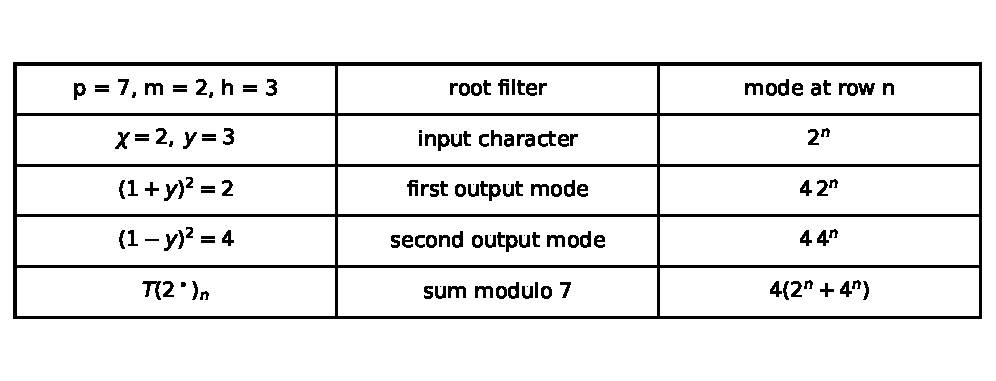
\includegraphics[width=.95\linewidth,height=3.15in,keepaspectratio]{../../figures/reconstructed/standard_fourier.pdf}
\caption{New reconstruction. Finite field Fourier transfer for a standard window. Each character becomes a finite sum of positive index modes with period dividing \(h\).}
\label{hist:fig:standard_fourier}
\end{figure}
\begin{figure}[t]
\centering
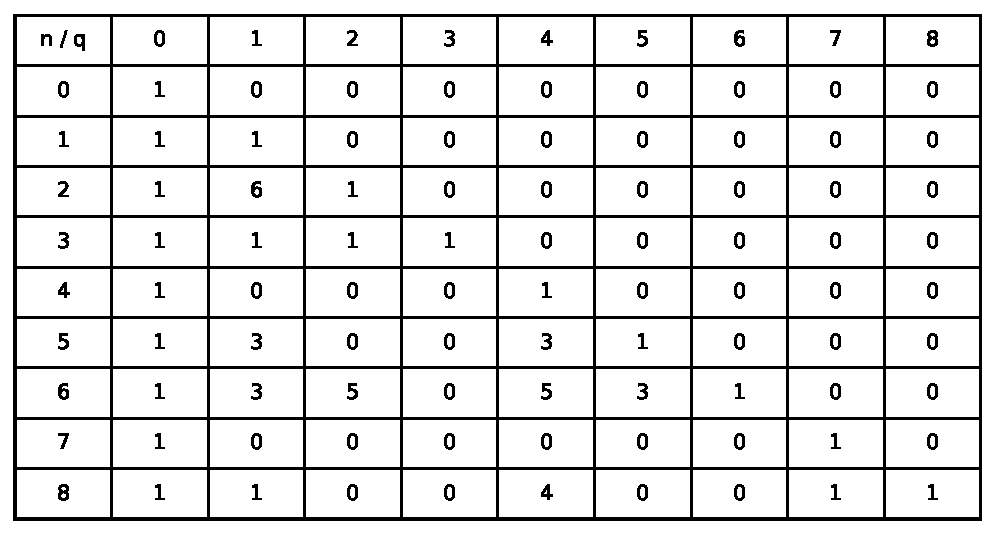
\includegraphics[width=.95\linewidth,height=3.15in,keepaspectratio]{../../figures/reconstructed/standard_matrix.pdf}
\caption{New reconstruction. The standard window matrix for $p=7$, $m=2$, and $0\le j<7$. Reduction removes the address and retains diagonal one.}
\label{hist:fig:standard_matrix}
\end{figure}

\begin{histremark}\label{hist:rem:period_boundary}
The theorem gives a period modulo \(p\). A period modulo higher powers requires additional control of the triangular inverse and cannot be inferred from the finite field argument alone.

\end{histremark}

\subsection{One local Euler source and kernel calculus}\label{hist:sec:local_euler}

The odd and dyadic reconstructions have one convolutional form. Their sources, kernels, and valuation profiles are different. We first construct each chart and then state the common theorem.

\subsubsection{The odd source and its inverse}

Let \(q\) be a positive odd integer. Define
\[
S_n(q)
=
\sum_{a=0}^{q-1}
(-1)^a(2a+1)^n.
\]
Let the signed Euler numbers and Euler zigzag numbers be defined by
\[
\operatorname{sech}t
=
\sum_{n\geq0}E_n\frac{t^n}{n!}
\]
and
\[
\sec t+\tan t
=
\sum_{n\geq0}Z_n\frac{t^n}{n!}.
\]

\begin{histlemma}[Odd source generating function]\label{hist:lem:odd_source_egf}
For every positive odd \(q\),
\[
\boxed{
\sum_{n\geq0}S_n(q)\frac{t^n}{n!}
=
\e^{qt}\cosh(qt)\operatorname{sech}t.
}
\]
Its even part is
\[
\boxed{
\sum_{n\geq0}S_{2n}(q)\frac{t^{2n}}{(2n)!}
=
\cosh^2(qt)\operatorname{sech}t.
}
\]
\end{histlemma}

\begin{proof}
The finite geometric sum gives
\[
\sum_{a=0}^{q-1}(-1)^a\e^{(2a+1)t}
=
\e^t\frac{1+\e^{2qt}}{1+\e^{2t}}
=
\e^{qt}\cosh(qt)\operatorname{sech}t.
\]
Averaging at \(t\) and \(-t\) gives the even part.
\end{proof}

\begin{histlemma}[Zigzag inverse kernel]\label{hist:lem:local_zigzag_kernel}
\[
\boxed{
\operatorname{sech}^2t
=
\sum_{r\geq0}
(-1)^rZ_{2r+1}
\frac{t^{2r}}{(2r)!}.
}
\]
\end{histlemma}

\begin{proof}
The identity \(\tanh t=-i\tan(it)\) gives the odd zigzag expansion of \(\tanh t\). Differentiate.
\end{proof}

\begin{histtheorem}[Odd modulus Euler coordinate pair]\label{hist:thm:odd_coordinate_pair}
For every positive odd \(q\) and every even \(n\geq0\),
\[
\boxed{
E_n
=
\sum_{r=0}^{n/2}
(-1)^rZ_{2r+1}
\binom n{2r}
q^{2r}S_{n-2r}(q).
}
\]
The inverse transform is
\[
\boxed{
S_n(q)
=
E_n
+
\sum_{r=1}^{n/2}
2^{2r-1}
\binom n{2r}
q^{2r}E_{n-2r}.
}
\]
Both transforms are lower triangular with diagonal one.
\end{histtheorem}

\begin{proof}
The even source identity gives
\[
\operatorname{sech}t
=
\operatorname{sech}^2(qt)
\sum_{n\geq0}S_{2n}(q)\frac{t^{2n}}{(2n)!}.
\]
Insert \cref{hist:lem:local_zigzag_kernel} and compare coefficients. For the inverse, multiply \(\operatorname{sech}t\) by
\[
\cosh^2(qt)
=
1+
\sum_{r\geq1}2^{2r-1}q^{2r}\frac{t^{2r}}{(2r)!}.
\]
\end{proof}

\begin{histcorollary}[Odd modulus truncation]\label{hist:cor:odd_modulus_truncation}
For every \(M\geq0\), every positive odd \(q\), and every even \(n\),
\[
\boxed{
E_n
\equiv
\sum_{r=0}^{\min(M,n/2)}
(-1)^rZ_{2r+1}
\binom n{2r}q^{2r}S_{n-2r}(q)
\pmod {q^{2M+2}}.
}
\]
If \(p\mid q\) and \(a=\vp(q)\), the same truncation is valid modulo \(p^{2a(M+1)}\).
\end{histcorollary}

\begin{proof}
Every omitted term contains \(q^{2r}\) with \(r\geq M+1\). The local statement follows by taking the \(p\) adic valuation.
\end{proof}

\begin{histproposition}[Odd row weight]\label{hist:prop:odd_row_weight}
For an odd prime \(p\), the \(r\)th nonzero term in the reconstruction has valuation
\[
\boxed{
W_p(n,r)
=
2r+\vp(Z_{2r+1})
+\vp\binom n{2r}
+\vp\bigl(S_{n-2r}(p)\bigr).
}
\]
The binomial contribution is
\[
\boxed{
\vp\binom n{2r}
=
\frac{s_p(2r)+s_p(n-2r)-s_p(n)}{p-1},
}
\]
where \(s_p\) is the base \(p\) digit sum.
\end{histproposition}

\begin{proof}
The first identity separates the valuation of every factor. The second is Legendre's formula, equivalently Kummer's carry theorem \cite{IrelandRosen1990}.
\end{proof}

\subsubsection{The dyadic source and its inverse}

For even \(n\geq0\), define
\[
\boxed{
R_n
=
\frac{3^{n+2}-1}{4(n+1)(n+2)}.
}
\]
Its even exponential generating function is
\[
\boxed{
\sum_{n\text{ even}}R_n\frac{t^n}{n!}
=
\frac{\sinh(2t)\sinh t}{2t^2}.
}
\]
Define \(\beta_r\) by
\[
\boxed{
\frac{z^2}{\sinh^2z}
=
\sum_{r\geq0}\beta_rz^{2r}.
}
\]

\begin{histproposition}[Dyadic inverse coefficients]\label{hist:prop:dyadic_beta_unified}
For \(r\geq1\),
\[
\boxed{
\beta_r
=
-
\frac{2^{2r}(2r-1)B_{2r}}{(2r)!}.
}
\]
Consequently,
\[
\boxed{
\vTwo(\beta_r)=\sTwo(r)-1.
}
\]
Every \(R_n\) is a dyadic unit.
\end{histproposition}

\begin{proof}
Differentiate the Bernoulli expansion of \(\coth z\) and use \(-(\coth z)'=\sinh(z)^{-2}\). The von Staudt and Clausen theorem gives \(\vTwo(B_{2r})=-1\). Legendre's formula gives
\[
\vTwo((2r)!)=2r-\sTwo(r).
\]
For \(R_n\), put \(k=n+2\). Since \(k\) is even,
\[
\vTwo(3^k-1)=2+\vTwo(k).
\]
The denominator has the same valuation because \(n+1\) is odd.
\end{proof}

\begin{histtheorem}[Dyadic Euler coordinate pair]\label{hist:thm:dyadic_coordinate_pair}
For every even \(n\geq0\),
\[
\boxed{
E_n
=
\sum_{r=0}^{n/2}
\beta_r2^{2r}
\fall n{2r}
R_{n-2r}.
}
\]
The inverse transform is
\[
\boxed{
R_n
=
\sum_{r=0}^{n/2}
\frac{2^{4r+1}}{(2r+2)!}
\fall n{2r}
E_{n-2r}.
}
\]
\end{histtheorem}

\begin{proof}
Substitute \(z=2t\) in the inverse series and multiply
\[
\frac{4t^2}{\sinh^2(2t)}
\frac{\sinh(2t)\sinh t}{2t^2}
=
\operatorname{sech}t.
\]
Coefficient extraction gives the forward transform. The inverse follows from
\[
\left(\frac{\sinh(2t)}{2t}\right)^2
=
\sum_{r\geq0}
\frac{2^{4r+1}}{(2r+2)!}t^{2r}.
\]
\end{proof}

\subsubsection{The common source and kernel law}

For a prime \(p\), define
\[
A_{p,n}
=
\begin{cases}
S_n(p),&p\text{ odd},\\
R_n,&p=2\text{ and }n\text{ even},\\
0,&p=2\text{ and }n\text{ odd},
\end{cases}
\]
and
\[
\kappa_{p,r}
=
\begin{cases}
(-1)^rZ_{2r+1}p^{2r},&p\text{ odd},\\
\beta_r2^{2r}(2r)!,&p=2.
\end{cases}
\]

\begin{histtheorem}[Unified local Euler transfer]\label{hist:thm:unified_local_euler}
For every prime \(p\) and every even \(n\geq0\),
\[
\boxed{
E_n
=
\sum_{r=0}^{n/2}
\binom n{2r}
\kappa_{p,r}
A_{p,n-2r}.
}
\]
If
\[
H_p(t)
=
\sum_{m\geq0}A_{p,2m}\frac{t^{2m}}{(2m)!}
\]
and
\[
K_p(t)
=
\sum_{r\geq0}\kappa_{p,r}\frac{t^{2r}}{(2r)!},
\]
then
\[
\boxed{K_p(t)H_p(t)=\operatorname{sech}t.}
\]
For odd \(p\),
\[
H_p(t)=\cosh^2(pt)\operatorname{sech}t,
\qquad
K_p(t)=\operatorname{sech}^2(pt).
\]
For \(p=2\),
\[
H_2(t)=\frac{\sinh(2t)\sinh t}{2t^2},
\qquad
K_2(t)=\frac{4t^2}{\sinh^2(2t)}.
\]
\end{histtheorem}

\begin{proof}
The two source and kernel products were proved in \cref{hist:thm:odd_coordinate_pair,hist:thm:dyadic_coordinate_pair}. Their divided power coefficient laws have the displayed common form.
\end{proof}

\begin{histtheorem}[Unified inverse local transfer]\label{hist:thm:unified_inverse_local_euler}
Define
\[
\lambda_{p,r}
=
\begin{cases}
1,&p\text{ odd and }r=0,\\
2^{2r-1}p^{2r},&p\text{ odd and }r\geq1,\\
\dfrac{2^{4r+1}}{(2r+1)(2r+2)},&p=2.
\end{cases}
\]
Then for every prime \(p\) and every even \(n\geq0\),
\[
\boxed{
A_{p,n}
=
\sum_{r=0}^{n/2}
\binom n{2r}
\lambda_{p,r}
E_{n-2r}.
}
\]
Equivalently, if
\[
L_p(t)=K_p(t)^{-1},
\]
then
\[
\boxed{H_p(t)=L_p(t)\operatorname{sech}t,}
\]
where
\[
L_p(t)=\cosh^2(pt)
\]
for odd \(p\), and
\[
L_2(t)=\left(\frac{\sinh(2t)}{2t}\right)^2
\]
for \(p=2\).
\end{histtheorem}

\begin{proof}
For odd \(p\), this is the inverse identity in \cref{hist:thm:odd_coordinate_pair}. For \(p=2\), rewrite the inverse identity in \cref{hist:thm:dyadic_coordinate_pair} by using
\[
\fall n{2r}=(2r)!\binom n{2r}.
\]
The coefficient becomes
\[
\frac{2^{4r+1}(2r)!}{(2r+2)!}
=
\frac{2^{4r+1}}{(2r+1)(2r+2)}.
\]
The generating functions are the inverses of the kernels in \cref{hist:thm:unified_local_euler}.
\end{proof}

\begin{histcorollary}[Exact change between local source charts]\label{hist:cor:local_source_change}
\par\noindent\textbf{Editorial range correction.} This comparison holds for the even source subsequences, equivalently the evenized generating functions $H_p$. It does not identify their full odd-degree source values. For $p=3$, the original odd source has $A_{3,1}=S_1(3)=3$, whereas every odd dyadic source coefficient is zero; the even kernel $L_3K_2$ cannot change that odd coefficient. Read the coefficient consequence below only at even indices. The displayed identity $H_p=L_pK_\ell H_\ell$ and its proof remain valid.\par\medskip
For any two primes \(p\) and \(\ell\), the source sequences \(A_{p,n}\) and \(A_{\ell,n}\) are related by an exact unit lower triangular transformation obtained by composing the inverse kernel \(L_p\) with the reconstruction kernel \(K_\ell\).
\end{histcorollary}

\begin{proof}
Both source series reconstruct \(\operatorname{sech}t\). Hence
\[
H_p(t)=L_p(t)K_\ell(t)H_\ell(t).
\]
The multiplier has constant coefficient one, so \cref{hist:thm:exact_coefficient_transport} gives an exact unit lower triangular coordinate change.
\end{proof}

\begin{table}[t]
\centering
\caption{The common local Euler architecture and the parts that remain prime dependent.}
\label{hist:tab:local_chart_comparison}
\begin{tabular}{>{\raggedright\arraybackslash}p{.22\textwidth}>{\raggedright\arraybackslash}p{.31\textwidth}>{\raggedright\arraybackslash}p{.31\textwidth}}
\toprule
Feature & Odd prime chart & Dyadic chart\\
\midrule
Finite torsion address & Modulo \(p-1\) & Sign address modulo two\\
Principal units & \(1+p\mathbb Z_p\) & \(1+4\mathbb Z_2\)\\
Source & Alternating odd power sum \(S_n(p)\) & Weighted source \(R_n\)\\
Kernel & \(\operatorname{sech}^2(pt)\) & \(4t^2/\sinh^2(2t)\)\\
Positive depth weight & At least \(2r\), with zigzag and row factors & Exactly \(4r-1\), before the binomial carry\\
Analytic branch & Depleted unit source & Direct integral source\\
Natural refined step & \((p-1)p^a\) & \(2^{a+1}\)\\
\bottomrule
\end{tabular}
\end{table}

\begin{histexample}[The first odd reconstruction]\label{hist:ex:first_odd_reconstruction}
For \(p=3\) and \(n=2\),
\[
S_2(3)=1-9+25=17.
\]
Since \(Z_1=1\), \(Z_3=2\), and \(S_0(3)=1\), the odd coordinate formula gives
\[
E_2
=17-2\cdot9
=-1.
\]
The large source value and the depth one correction are both necessary.
\end{histexample}

\begin{histexample}[The first nontrivial dyadic row]\label{hist:ex:first_dyadic_reconstruction}
For \(n=4\),
\[
R_4=\frac{91}{15},
\qquad
R_2=\frac53,
\qquad
R_0=1.
\]
The exact kernel coefficients are
\[
\kappa_{2,1}=-\frac83,
\qquad
\kappa_{2,2}=\frac{128}{5}.
\]
Therefore
\[
E_4
=
\frac{91}{15}
-\frac83\binom42\frac53
+\frac{128}{5}
=5.
\]
The rational source values are dyadic units, while the transfer depth is carried by the kernel.
\end{histexample}

\begin{histremark}\label{hist:rem:no_dyadic_substitution}
The common convolution does not identify the integral charts. At an odd prime the finite character coordinate has order \(p-1\). At the dyadic prime it begins with the sign coordinate, and the principal unit subgroup begins at \(1+4\mathbb Z_2\).
\end{histremark}

\subsubsection{Exact dyadic transfer depth}

For \(r\geq1\), write
\[
\kappa_{2,r}
=
\beta_r2^{2r}(2r)!
=
-2^{4r}(2r-1)B_{2r}.
\]

\begin{histtheorem}[Exact dyadic kernel weight]\label{hist:thm:exact_dyadic_kernel_weight}
\par\noindent\textbf{Editorial index conventions.} The standalone kernel valuation holds for all $r\ge1$. Its reconstruction-term formula requires even $n\ge0$ and $1\le r\le n/2$. In the following truncation formulas only terms with $r\le n/2$ occur; terms that would use $R_{n-2r}$ at a negative index are omitted. An empty tail is exactly zero, and the minimum over an empty set of term valuations is $+\infty$. These conventions include $M\ge n/2$.\par\medskip
For every \(r\geq1\),
\[
\boxed{\vTwo(\kappa_{2,r})=4r-1.}
\]
The \(r\)th reconstruction term has exact valuation
\[
\boxed{
\vTwo\left(
\kappa_{2,r}\binom n{2r}R_{n-2r}
\right)
=
4r-1+\vTwo\binom n{2r}.
}
\]
Equivalently,
\[
\boxed{
W_2(n,r)
=
4r-1+\sTwo(r)+\sTwo(n-2r)-\sTwo(n).
}
\]
\end{histtheorem}

\begin{proof}
The Bernoulli formula gives \(\vTwo(B_{2r})=-1\). The source value is a unit. Kummer's binary carry formula gives the last expression.
\end{proof}

\begin{histtheorem}[Optimal dyadic truncation]\label{hist:thm:optimal_dyadic_truncation}
Let
\[
T_{2,M}(n)
=
\sum_{r=0}^{\min(M,n/2)}
\kappa_{2,r}\binom n{2r}R_{n-2r}.
\]
Then
\[
\boxed{
E_n\equiv T_{2,M}(n)\pmod {2^{4M+3}}.
}
\]
More precisely,
\[
\boxed{
\vTwo\bigl(E_n-T_{2,M}(n)\bigr)
\geq
\min_{M+1\leq r\leq n/2}
\left(
4r-1+\vTwo\binom n{2r}
\right).
}
\]
The uniform exponent \(4M+3\) is best possible.
\end{histtheorem}

\begin{proof}
Every omitted term has valuation at least \(4(M+1)-1\). For optimality, take \(n=2M+2\). There is one omitted term. Its binomial coefficient and source value are one, so its valuation is exactly \(4M+3\).
\end{proof}

The first three sharp truncations are
\[
\begin{aligned}
E_n&\equiv R_n&&\pmod 8,\\
E_n&\equiv R_n-\frac83\binom n2R_{n-2}&&\pmod {128},\\
E_n&\equiv R_n-\frac83\binom n2R_{n-2}
+\frac{128}{5}\binom n4R_{n-4}&&\pmod {2048}.
\end{aligned}
\]

\begin{figure}[t]
\centering
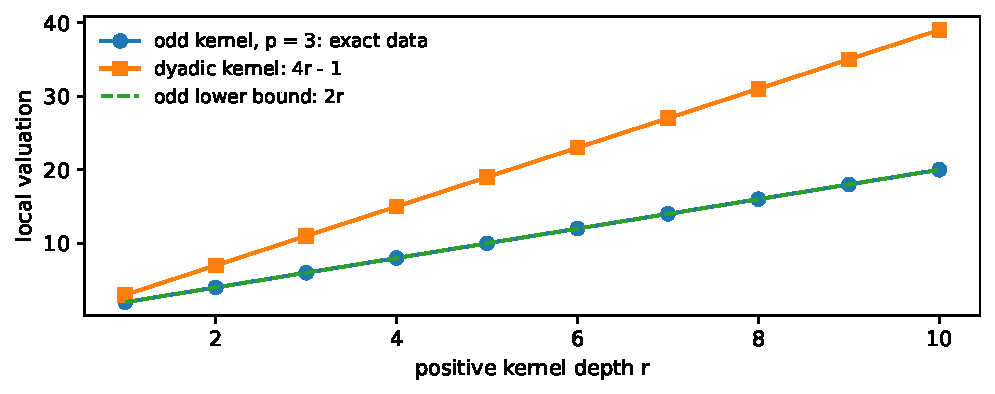
\includegraphics[width=.95\linewidth,height=3.15in,keepaspectratio]{../../figures/reconstructed/local_kernel_weights.pdf}
\caption{New reconstruction. Odd and dyadic kernels share one convolution law but have different valuation profiles. The positive depth dyadic kernel has exact slope four and offset minus one.}
\label{hist:fig:local_kernel_weights}
\end{figure}

\begin{figure}[t]
\centering
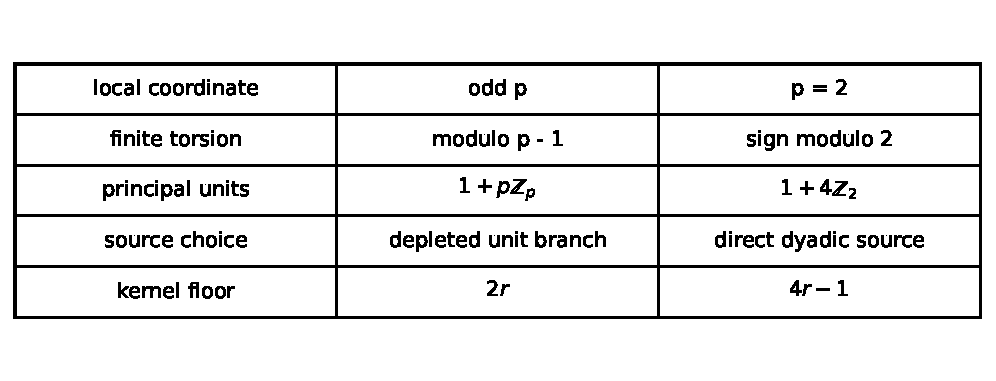
\includegraphics[width=.95\linewidth,height=3.15in,keepaspectratio]{../../figures/reconstructed/odd_dyadic_geometry.pdf}
\caption{New reconstruction. The local Euler charts share source and kernel reconstruction. Their torsion addresses, principal unit depths, source corrections, and precision growth remain different.}
\label{hist:fig:odd_dyadic_geometry}
\end{figure}
\subsection{Mahler transfer and local analytic branches}\label{hist:sec:mahler}

The finite character coordinate resolves the torsion part of a local unit. A sufficiently long arithmetic jump moves the remaining unit into a principal unit neighborhood. The coarse variable then has a convergent Mahler expansion with an explicit valuation slope.

\subsubsection{Finite Mahler coordinates}

For a function \(f\) on the nonnegative integers, define
\[
\Delta f(n)=f(n+1)-f(n).
\]

\begin{histtheorem}[Finite Mahler reconstruction]\label{hist:thm:finite_mahler_unified}
Given \(f(0),\ldots,f(N)\), put \(c_r=\Delta^rf(0)\). Then
\[
\boxed{
f(n)=\sum_{r=0}^{n}c_r\binom nr
\qquad(0\leq n\leq N).
}
\]
For every \(s\) with \(0\leq s\leq N\),
\[
\boxed{
\Delta^sf(n)
=
\sum_{r=s}^{N}c_r\binom n{r-s}
\qquad(0\leq n\leq N-s).
}
\]
\end{histtheorem}

\begin{proof}
Let
\[
P(x)=\sum_{r=0}^{N}c_r\binom xr.
\]
Newton interpolation gives \(P(n)=f(n)\) for \(0\leq n\leq N\). Iterating
\[
\Delta\binom xr=\binom x{r-1}
\]
gives
\[
\Delta^sP(n)=\sum_{r=s}^{N}c_r\binom n{r-s}.
\]
When \(0\leq n\leq N-s\), every value used in \(\Delta^sf(n)\) lies among the prescribed data, so \(\Delta^sf(n)=\Delta^sP(n)\).
\end{proof}

\begin{histcorollary}[Mahler valuation ledger]\label{hist:cor:mahler_valuation_ledger}
If \(c_r\in\Zp\) and \(\vp(c_r)\geq w(r)\), then
\[
\boxed{
\vp(\Delta^sf(n))
\geq
\min_{r\geq s}
\left(
w(r)+\vp\binom n{r-s}
\right).
}
\]
\end{histcorollary}

\begin{proof}
Apply the nonarchimedean triangle inequality to \cref{hist:thm:finite_mahler_unified}.
\end{proof}

The infinite interpolation theorem states that every continuous function on \(\Zp\) has a unique convergent Mahler expansion \cite{Mahler1958,Robert2000}. We use that theorem as a standard input when the local variable is allowed to range over all of \(\Zp\).

\subsubsection{Carmichael and Mahler transfer for unit modes}

\begin{histstandardfact}[Local unit decomposition]\label{hist:fact:local_unit_decomposition}
For odd \(p\), every unit has a unique factorization
\[
u=\omega(u)\langle u\rangle,
\qquad
\omega(u)^{p-1}=1,
\qquad
\langle u\rangle\in1+p\mathbb Z_p.
\]
Every dyadic unit has a unique factorization
\[
u=(-1)^{\epsilon(u)}\langle u\rangle,
\qquad
\epsilon(u)\in\{0,1\},
\qquad
\langle u\rangle\in1+4\mathbb Z_2.
\]
The first factor gives the finite character address. The second factor admits logarithmic and Mahler coordinates.
\end{histstandardfact}

For odd \(p\) and \(L\geq1\), put
\[
\Lambda_{p,L}=(p-1)p^{L-1}.
\]
For \(p=2\) and \(L\geq3\), put
\[
\Lambda_{2,L}=2^{L-2}.
\]
These are exponents of the unit groups modulo the declared prime powers.

\begin{histtheorem}[One unit mode]\label{hist:thm:carmichael_mahler_scalar}
Let \(u\in\Zp^\times\), let \(H=\Lambda_{p,L}\), and put
\[
q_{u,L}=u^H-1\in p^L\Zp.
\]
For every integer address \(j\) and every \(x\in\Zp\),
\[
\boxed{
u^{Hx+j}
=
u^j\sum_{r\geq0}q_{u,L}^{\,r}\binom xr.
}
\]
The \(r\)th Mahler coefficient has valuation at least \(Lr\).
\end{histtheorem}

\begin{proof}
Write \(u^{Hx+j}=u^j(1+q_{u,L})^x\) and use the convergent binomial series on \(\Zp\).
\end{proof}

\begin{histexample}[Paired principal unit expansions]\label{hist:ex:paired_unit_expansions}
At the odd prime three,
\[
2^{2x+j}
=
2^j4^x
=
2^j\sum_{r\geq0}3^r\binom xr.
\]
At the dyadic prime,
\[
3^{2x+j}
=
3^j9^x
=
3^j\sum_{r\geq0}8^r\binom xr.
\]
The formal expansions are identical. Their first local slopes are one and three because \(4-1=3\) while \(9-1=8\).
\end{histexample}

\begin{histcorollary}[Basic odd and dyadic difference gains]\label{hist:cor:basic_local_difference_gains}
For odd \(p\),
\[
\boxed{
\Delta_{(p-1)p^a}^{\,r}u^n
=
u^n\left(u^{(p-1)p^a}-1\right)^r,
\qquad
\vp\left(\Delta_{(p-1)p^a}^{\,r}u^n\right)\geq(a+1)r.
}
\]
For odd \(u\in\mathbb Z_2^\times\),
\[
\boxed{
\Delta_{2^{a+1}}^{\,r}u^n
=
u^n\left(u^{2^{a+1}}-1\right)^r,
\qquad
\vTwo\left(\Delta_{2^{a+1}}^{\,r}u^n\right)\geq(a+3)r.
}
\]
\end{histcorollary}

\begin{proof}
One step difference multiplies a unit mode by \(u^H-1\). Fermat reduction and lifting the exponent give the odd estimate. For odd \(u\),
\[
\vTwo\left(u^{2^{a+1}}-1\right)
=
\vTwo(u^2-1)+a
\geq a+3.
\]
\end{proof}

\subsubsection{Polynomial exponential modes}

\begin{histtheorem}[Polynomial exponential Mahler transfer]\label{hist:thm:polynomial_exponential_mahler}
Let
\[
f(n)=P(n)u^n
\]
with \(P\in\Zp[n]\) of degree \(d\). Let \(H=\Lambda_{p,L}\), fix an address \(j\), and write
\[
Q_j(x)=P(Hx+j),
\qquad
y=u^H,
\qquad q=y-1.
\]
Then
\[
\boxed{
f(Hx+j)=\sum_{r\geq0}c_{j,r}\binom xr,
}
\]
where
\[
\boxed{
c_{j,r}
=
u^j
\sum_{k=0}^{\min(d,r)}
\binom rk
\Delta^kQ_j(0)y^kq^{r-k}.
}
\]
Consequently,
\[
\boxed{
\vp(c_{j,r})\geq L\max(r-d,0).
}
\]
For \(R\geq d\), truncation at depth \(R\) is valid modulo \(p^{L(R+1-d)}\) uniformly on \(\Zp\).
\end{histtheorem}

\begin{proof}
On the polynomial factor the difference operator acts as \(q+y\Delta\). The two terms commute. Expand \((q+y\Delta)^r\) and evaluate at zero. Since \(\Delta^kQ_j=0\) for \(k>d\), every surviving term contains at least \(q^{r-d}\).
\end{proof}

\subsubsection{Matrix state systems and finite adelic synchronization}

Let
\[
v_{n+1}=Cv_n,
\qquad
a_n=w^TC^nv_0,
\]
with \(C\in M_d(\Zp)\) invertible modulo \(p\).

\begin{histtheorem}[Matrix Carmichael and Mahler transfer]\label{hist:thm:matrix_carmichael_mahler}
\par\noindent\textbf{Editorial hypothesis correction.} The original displayed statement leaves the vectors untyped. Its integrality conclusion requires $v_0,w\in\Z_p^d$, $L\ge1$, and $H,j,n\in\N$ with $H>0$; the value at $Hx+j$ for $x\in\Z_p$ means the matrix-binomial interpolation. With $p=3$, $C=4$, $L=1$, $w=1$ and $v_0=1/3$, one has $\Delta_1a_0=1$, which is not in $3\Z_3$. The printed claim without these restrictions is therefore not an as-written certificate. The full original proof follows under the corrected hypotheses.\par\medskip
Assume
\[
C^H=I+p^LB
\]
with \(B\in M_d(\Zp)\). For every address \(j\) and every \(x\in\Zp\),
\[
\boxed{
a_{Hx+j}
=
\sum_{r\geq0}
p^{Lr}\binom xr
w^TC^jB^rv_0.
}
\]
The series converges on \(\Zp\), and
\[
\boxed{
\Delta_H^ra_n
\equiv0
\pmod {p^{Lr}}.
}
\]
\end{histtheorem}

\begin{proof}
Use
\[
C^{Hx+j}=C^j(I+p^LB)^x
\]
and the matrix binomial series. One difference in the coarse variable multiplies the series by \(p^LB\).
\end{proof}

\begin{histtheorem}[Finite adelic transfer]\label{hist:thm:finite_adelic_transfer}
\par\noindent\textbf{Editorial hypothesis correction.} Read this statement with $v_0,w\in\Z^d$, $H>0$ and $j,n,r\in\N$, and positive integer $L_p$. These restrictions make the integral congruences and powers well typed. Allowing $v_0=1/3$ in the one-prime example above loses the advertised digit; invertibility of $C$ alone does not restore it. The original proof is retained under these hypotheses.\par\medskip
Let
\[
Q=\prod_{p\in S}p^{L_p}
\]
for a finite set of primes. Let \(C\in M_d(\ZZ)\) be invertible modulo \(Q\), and choose \(H\) such that
\[
C^H=I+QB
\]
with \(B\in M_d(\ZZ)\). Then for every nonnegative integer \(x\),
\[
\boxed{
a_{Hx+j}
=
\sum_{r=0}^{x}Q^r\binom xr
w^TC^jB^rv_0.
}
\]
For every \(r\),
\[
\boxed{
\Delta_H^ra_n\equiv0\pmod {Q^r}.
}
\]
\end{histtheorem}

\begin{proof}
Apply the integer matrix binomial theorem and reduce at every selected prime.
\end{proof}

\begin{histexample}[A simultaneous Fibonacci jump]\label{hist:ex:fibonacci_finite_adelic}
Let
\[
C=
\begin{pmatrix}
1&1\\
1&0
\end{pmatrix}.
\]
The matrix \(C\) is invertible modulo twenty four, and
\[
C^{24}-I
=
24
\begin{pmatrix}
3126&1932\\
1932&1194
\end{pmatrix}.
\]
For every scalar coordinate of the state sequence \(C^nv_0\),
\[
\boxed{
\Delta_{24}^{\,r}a_n
\equiv0
\pmod {24^r}.
}
\]
One integral jump therefore gives simultaneous congruence ladders at the primes two and three.
\end{histexample}

\subsubsection{Amice pullback}

\begin{histdefinition}[Amice pullback]\label{hist:def:amice_pullback_unified}
For a formal exponential generating series
\[
F(z)=\sum_{n\geq0}a_n\frac{z^n}{n!},
\]
define
\[
\widehat F(T)=F(\log(1+T)).
\]
\end{histdefinition}

\begin{histtheorem}[Derivative conjugacy]\label{hist:thm:amice_derivative_unified}
\[
\boxed{
\widehat{F'}(T)
=
(1+T)\frac{d}{dT}\widehat F(T).
}
\]
\end{histtheorem}

\begin{proof}
Differentiate the composition \(F(\log(1+T))\).
\end{proof}

\begin{histproposition}[Weighted convergence]\label{hist:prop:amice_weighted_convergence_unified}
If
\[
\widehat F(T)=\sum_{r\geq0}c_rT^r
\]
and
\[
\vp(c_r)+r\alpha\longrightarrow+\infty,
\]
then the series converges whenever \(\vp(T)\geq\alpha\).
\end{histproposition}

\begin{proof}
The valuation of the \(r\)th term is \(\vp(c_r)+r\vp(T)\), which tends to positive infinity.
\end{proof}

\subsubsection{Odd prime depletion}

For an odd prime \(p\), the source \(S_n(p)\) contains one nonunit base. Put
\[
\sigma_p=(-1)^{(p-1)/2}
\]
and
\[
S_n^\times(p)=S_n(p)-\sigma_pp^n.
\]

\begin{histtheorem}[Depleted odd prime reconstruction]\label{hist:thm:depleted_odd_reconstruction}
For every even \(n\),
\[
\boxed{
\left(1-\sigma_pp^n\right)E_n
=
\sum_{r=0}^{n/2}
(-1)^rZ_{2r+1}
\binom n{2r}p^{2r}S_{n-2r}^\times(p).
}
\]
\end{histtheorem}

\begin{proof}
The removed source mode contributes \(\sigma_p\cosh(pt)\). Multiplication by \(\operatorname{sech}^2(pt)\) gives \(\sigma_p\operatorname{sech}(pt)\). Subtract it from the full source and kernel product.
\end{proof}

Fix an even address \(j\in\{0,2,\ldots,p-3\}\). For \(x\in\Zp\), define
\[
\begin{aligned}
\mathscr E_{p,j}^\times(x)
=
\sum_{r\geq0}
&(-1)^rZ_{2r+1}p^{2r}
\binom{(p-1)x+j}{2r}\\
&\times
\sum_{\substack{0\leq a<p\\2a+1\neq p}}
(-1)^a
(2a+1)^{j-2r}
\left((2a+1)^{p-1}\right)^x.
\end{aligned}
\]

\begin{histtheorem}[Odd prime analytic Euler branch]\label{hist:thm:odd_analytic_branch}
The series defining \(\mathscr E_{p,j}^\times\) converges in the Tate algebra on \(\Zp\). For every nonnegative integer \(x\),
\[
\boxed{
\mathscr E_{p,j}^\times(x)
=
\left(1-\sigma_pp^{(p-1)x+j}\right)
E_{(p-1)x+j}.
}
\]
\end{histtheorem}

\begin{proof}
Every retained base is a unit, and its \((p-1)\)st power lies in \(1+p\Zp\). The polynomial
\[
p^{2r}\binom{(p-1)x+j}{2r}
\]
has Gauss norm at most
\[
p^{-2r+\vp((2r)!)}.
\]
This tends to zero because \(p\) is odd. The remaining factors have bounded Gauss norm. Thus the series converges in the Tate algebra. At a nonnegative integer \(x\), the binomial factor vanishes for large \(r\), and \cref{hist:thm:depleted_odd_reconstruction} gives the value.
\end{proof}

\begin{histremark}\label{hist:rem:depleted_factor_boundary}
The analytic function is defined by its unit source series. The expression \(p^{(p-1)x+j}\) in the interpolation identity is evaluated only at nonnegative integers. No analytic function \(x\mapsto p^x\) on all of \(\Zp\) is used.
\end{histremark}

\subsubsection{Direct dyadic interpolation}

For \(x\in\mathbb Z_2\), define
\[
\boxed{
\mathscr R(x)
=
\frac{9^{x+1}-1}{8(x+1)(2x+1)}.
}
\]
The apparent singularity at \(x=-1\) is removable, with value \(-\log(9)/8\).

\begin{histlemma}[Analytic dyadic source]\label{hist:lem:analytic_dyadic_source}
The function \(\mathscr R\) belongs to the dyadic Tate algebra and takes values in \(\mathbb Z_2\). For every nonnegative integer \(n\),
\[
\boxed{\mathscr R(n)=R_{2n}.}
\]
\end{histlemma}

\begin{proof}
Put \(y=x+1\) and let \(\ell=\log 9\). Since \(\vTwo(\ell)=3\),
\[
\frac{9^y-1}{8y}
=
\frac{\ell}{8}
\sum_{m\geq0}
\frac{\ell^m}{(m+1)!}y^m.
\]
The coefficient of \(y^m\) has valuation
\[
3m-\vTwo((m+1)!),
\]
which is nonnegative and tends to positive infinity. The quotient therefore belongs to \(\mathbb Z_2\langle y\rangle\). The factor \(2x+1=1+2x\) is a unit in \(\mathbb Z_2\langle x\rangle\), with inverse \(\sum_{m\geq0}(-2x)^m\). Hence \(\mathscr R\) is integral and analytic. The integer values follow from the definition of \(R_{2n}\).
\end{proof}

Define
\[
\boxed{
\mathscr E_2(x)
=
\sum_{r\geq0}
\kappa_{2,r}
\binom{2x}{2r}
\mathscr R(x-r).
}
\]

\begin{histtheorem}[Direct dyadic Euler interpolation]\label{hist:thm:direct_dyadic_interpolation}
The series defining \(\mathscr E_2\) converges in the dyadic Tate algebra. For every nonnegative integer \(n\),
\[
\boxed{\mathscr E_2(n)=E_{2n}.}
\]
Truncation after depth \(M\) is uniformly valid modulo \(2^{4M+3}\) on \(\mathbb Z_2\).
\end{histtheorem}

\begin{proof}
The monomial Gauss norm of \(\binom{2x}{2r}\) is at most \(2^{\vTwo((2r)!)}\). Since
\[
\vTwo(\kappa_{2,r})=4r-1,
\]
the product tends to zero in Gauss norm. Translation by the integer \(r\) preserves the unit disc, so \(\mathscr R(x-r)\) remains an integral analytic function with uniformly bounded supremum norm. The series therefore converges in the Tate algebra.

At a nonnegative integer \(n\), every term with \(r>n\) vanishes and \cref{hist:thm:dyadic_coordinate_pair} remains. For arbitrary \(x\in\mathbb Z_2\), the integer valued polynomial \(\binom{2x}{2r}\) and the source value \(\mathscr R(x-r)\) lie in \(\mathbb Z_2\). Every omitted term after depth \(M\) is therefore divisible by \(2^{4M+3}\). This proves the uniform truncation statement.
\end{proof}

\begin{histtheorem}[Unified local interpolation statement]\label{hist:thm:unified_local_interpolation}
The odd branch \(\mathscr E_{p,j}^\times\) and the dyadic branch \(\mathscr E_2\) are analytic local realizations of the source and kernel law in \cref{hist:thm:unified_local_euler}. At integer arguments they recover, respectively,
\[
\left(1-\sigma_pp^n\right)E_n
\]
on each even odd prime character branch and
\[
E_{2n}
\]
on the dyadic even branch. The two realizations have distinct source corrections and distinct kernel valuation slopes.
\end{histtheorem}

\begin{proof}
Combine \cref{hist:thm:odd_analytic_branch,hist:thm:direct_dyadic_interpolation} with the source and kernel definitions in \cref{hist:thm:unified_local_euler}.
\end{proof}

\subsection{Polyphase refinement of local Mahler coordinates}\label{hist:sec:polyphase}

Polyphase refinement replaces one local branch by finitely many digit branches while preserving exact synthesis. For sequences it is residue analysis. For local functions it is the digit tree of \(\mathbb Z_p\). In Mahler coordinates it becomes a finite triangular kernel.

\subsubsection{Discrete analysis and exact synthesis}

For a sequence \(a=(a_n)_{n\geq0}\) and \(M\geq2\), define
\[
a_r^{[M]}(q)=a_{Mq+r}
\qquad(0\leq r<M).
\]
The analysis map is
\[
\mathcal P_Ma
=
\left(a_0^{[M]},\ldots,a_{M-1}^{[M]}\right).
\]
Synthesis interleaves the branches by the rule
\[
a_{Mq+r}=a_r^{[M]}(q).
\]

\begin{histtheorem}[Exact discrete polyphase reconstruction]\label{hist:thm:discrete_polyphase_reconstruction}
The analysis map \(\mathcal P_M\) is a bijection between sequences and ordered families of \(M\) sequences. If
\[
A(z)=\sum_{n\geq0}a_nz^n
\]
and
\[
A_r^{[M]}(w)=\sum_{q\geq0}a_{Mq+r}w^q,
\]
then
\[
\boxed{
A(z)=\sum_{r=0}^{M-1}z^rA_r^{[M]}(z^M).
}
\]
\end{histtheorem}

\begin{proof}
Every nonnegative integer has a unique expression \(Mq+r\) with \(0\leq r<M\). Group the terms of the ordinary generating function by this residue.
\end{proof}

\begin{histtheorem}[Nested discrete refinement]\label{hist:thm:nested_discrete_polyphase}
For positive integers \(M,N\),
\[
\boxed{
\left(a_r^{[M]}\right)_s^{[N]}
=
a_{r+Ms}^{[MN]}.
}
\]
For a mixed radix path \((M_1,\ldots,M_\ell)\) with digits \(0\leq s_i<M_i\), the final address is
\[
\boxed{
r(\boldsymbol s)
=
s_1+M_1s_2+\cdots+
\left(\prod_{i=1}^{\ell-1}M_i\right)s_\ell.
}
\]
Only the product radix and accumulated address determine the final branch.
\end{histtheorem}

\begin{proof}
Direct substitution gives
\[
\left(a_r^{[M]}\right)_s^{[N]}(q)
=
a_{M(Nq+s)+r}.
\]
Iterate this identity along the mixed radix path.
\end{proof}

\subsubsection{Carry convolution and the shift matrix}

Let \(c=a*b\) be the ordinary Cauchy convolution. Write \(A_r\), \(B_r\), and \(C_r\) for the phase ordinary generating functions.

\begin{histproposition}[One carry convolution law]\label{hist:prop:polyphase_carry_convolution}
For every residue \(r\),
\[
\boxed{
C_r(w)
=
\sum_{u+v=r}A_u(w)B_v(w)
+
w\sum_{u+v=r+M}A_u(w)B_v(w).
}
\]
The first sum has no phase carry. The second has one coarse index carry.
\end{histproposition}

\begin{proof}
Write the input indices as \(Mq+u\) and \(Mq'+v\). Since \(0\leq u,v<M\), their sum has residue \(u+v\) when \(u+v<M\), and residue \(u+v-M\) with one additional coarse index when \(u+v\geq M\).
\end{proof}

\begin{histtheorem}[Polyphase shift matrix]\label{hist:thm:polyphase_shift_matrix}
Let \(E\) be the scalar shift \((Ea)_n=a_{n+1}\), and let \(E_q\) shift the coarse index. Then
\[
\boxed{
\mathcal P_M(Ea)
=
\mathsf S_M(E_q)\mathcal P_Ma,
}
\]
where
\[
\mathsf S_M(E_q)
=
\begin{pmatrix}
0&1&0&\cdots&0\\
0&0&1&\cdots&0\\
\vdots&&&\ddots&\vdots\\
0&0&0&\cdots&1\\
E_q&0&0&\cdots&0
\end{pmatrix}.
\]
It also satisfies
\[
\boxed{\mathsf S_M(E_q)^M=E_qI_M.}
\]
\end{histtheorem}

\begin{proof}
For \(r<M-1\),
\[
(Ea)_{Mq+r}=a_{Mq+r+1}=a_{r+1}^{[M]}(q).
\]
For \(r=M-1\),
\[
(Ea)_{Mq+M-1}=a_{M(q+1)}=E_qa_0^{[M]}(q).
\]
After \(M\) shifts every phase has advanced by one coarse index.
\end{proof}

\subsubsection{Local branches and digit reconstruction}

For \(a\geq1\) and \(0\leq s<p^a\), define
\[
f_{a,s}(x)=f(p^ax+s).
\]

\begin{histtheorem}[Exact local branch reconstruction]\label{hist:thm:local_branch_reconstruction}
The family \(\{f_{a,s}\}_{0\leq s<p^a}\) determines \(f\) uniquely on \(\mathbb Z_p\). More precisely, if \(y\in s+p^a\mathbb Z_p\), then
\[
\boxed{
f(y)=f_{a,s}\left(\frac{y-s}{p^a}\right).
}
\]
For \(a,b\geq1\),
\[
\boxed{
(f_{a,s})_{b,t}
=
f_{a+b,s+p^at}.
}
\]
Thus local refinement is exactly the \(p\) adic digit tree.
\end{histtheorem}

\begin{proof}
The cosets \(s+p^a\mathbb Z_p\) form a disjoint partition of \(\mathbb Z_p\). The first formula is the inverse affine change of variables on one coset. The second follows from
\[
p^a(p^bx+t)+s
=
p^{a+b}x+p^at+s.
\]
\end{proof}

\subsubsection{The affine Mahler kernel}

Let
\[
\Phi_M(z)=(1+z)^M-1.
\]
For \(M\geq1\), \(s\geq0\), and \(r,k\geq0\), define
\[
\boxed{
\Theta_{M,s}(r,k)
=
[z^r](1+z)^s\Phi_M(z)^k.
}
\]
Equivalently,
\[
\boxed{
\Theta_{M,s}(r,k)
=
\sum_{j=0}^{k}
(-1)^{k-j}\binom kj\binom{Mj+s}{r}.
}
\]
It vanishes unless
\[
k\leq r\leq Mk+s.
\]

\begin{histproposition}[Edge coefficients of the affine kernel]\label{hist:prop:affine_kernel_edges}
For every \(M\geq1\), \(s\geq0\), and \(k\geq0\),
\[
\boxed{
\Theta_{M,s}(k,k)=M^k,
\qquad
\Theta_{M,s}(Mk+s,k)=1.
}
\]
For binary radix and zero address,
\[
\boxed{
\Theta_{2,0}(k+j,k)
=
2^{k-j}\binom kj
\qquad(0\leq j\leq k).
}
\]
Hence
\[
\boxed{
\vTwo\left(\Theta_{2,0}(k+j,k)\right)
=
k-j+\vTwo\binom kj.
}
\]
\end{histproposition}

\begin{proof}
The lowest degree term of \(\Phi_M(z)\) is \(Mz\), and its highest degree term is \(z^M\). Multiplication by \((1+z)^s\) gives the two edge coefficients. When \(M=2\) and \(s=0\),
\[
\Phi_2(z)^k
=
(2z+z^2)^k
=
z^k(2+z)^k.
\]
Taking the coefficient of \(z^{k+j}\) gives the binary formula.
\end{proof}

\begin{histtheorem}[Mahler polyphase transfer]\label{hist:thm:mahler_polyphase_transfer}
Let
\[
f(x)=\sum_{r\geq0}c_r\binom xr
\]
be a convergent Mahler expansion. For
\[
g_s(q)=f(Mq+s),
\]
one has
\[
\boxed{
g_s(q)=\sum_{k\geq0}d_{s,k}\binom qk,}
\]
where
\[
\boxed{
d_{s,k}
=
\sum_{r=k}^{Mk+s}
c_r\Theta_{M,s}(r,k).
}
\]
Every refined coefficient uses a finite window of the original Mahler coefficients.
\end{histtheorem}

\begin{proof}
Use
\[
(1+z)^{Mq+s}
=
(1+z)^s\left(1+\Phi_M(z)\right)^q
=
\sum_{k\geq0}\binom qk(1+z)^s\Phi_M(z)^k.
\]
Taking the coefficient of \(z^r\) gives the affine expansion of \(\binom{Mq+s}{r}\). Since \(c_r\to0\) and every \(d_{s,k}\) uses indices \(r\geq k\), the transformed coefficients also tend to zero.
\end{proof}

\begin{histtheorem}[Kernel composition]\label{hist:thm:polyphase_kernel_composition}
For positive integers \(M,N\),
\[
\boxed{
\sum_{k\geq0}
\Theta_{M,s}(r,k)
\Theta_{N,t}(k,\ell)
=
\Theta_{MN,Mt+s}(r,\ell).
}
\]
The sum is finite.
\end{histtheorem}

\begin{proof}
Apply \cref{hist:thm:mahler_polyphase_transfer} first to \(x=Mq+s\) and then to \(q=Ny+t\). The composite substitution is \(x=MNy+Mt+s\). Uniqueness of Mahler coefficients gives the identity.
\end{proof}

\subsubsection{Valuation transport}

\begin{histtheorem}[Polyphase valuation ledger]\label{hist:thm:polyphase_valuation_ledger}
For every refined coefficient,
\[
\boxed{
\vp(d_{s,k})
\geq
\min_{k\leq r\leq Mk+s}
\left(
\vp(c_r)+\vp(\Theta_{M,s}(r,k))
\right).
}
\]
If \(\vp(c_r)\geq w(r)\) for a nondecreasing function \(w\), then
\[
\boxed{\vp(d_{s,k})\geq w(k).}
\]
Thus every monotone Mahler precision ladder survives arbitrary polyphase refinement.
\end{histtheorem}

\begin{proof}
Apply the nonarchimedean triangle inequality to the finite coefficient formula. Since \(r\geq k\), monotonicity gives \(w(r)\geq w(k)\), and the affine kernel is integral.
\end{proof}

\begin{histtheorem}[Prime power sparsification]\label{hist:thm:prime_power_sparsification}
\par\noindent\textbf{Editorial hypothesis correction.} The affine-kernel congruence below needs no change, but its consequence for transformed Mahler coefficients requires $c_r\in\Z_p$ for every $r$. Convergence of a $\Q_p$-valued Mahler expansion alone is insufficient. For $p=2$, $M=2$, $s=0$ and $f(x)=x/2$, one has $c_1=1/2$, $c_2=0$, while $g(q)=q$ has $d_1=1$; thus $d_1\not\equiv c_2\pmod2$. The coefficient consequence is read with integral original coefficients.\par\medskip
Let \(M=p^a\). Then
\[
\boxed{
\Theta_{p^a,s}(r,k)
\equiv
\binom{s}{r-p^ak}
\pmod p,
}
\]
where the binomial coefficient is zero outside its natural range. Consequently,
\[
\boxed{
d_{s,k}
\equiv
\sum_{u=0}^{s}
\binom su
c_{p^ak+u}
\pmod p.
}
\]
In particular,
\[
\boxed{d_{0,k}\equiv c_{p^ak}\pmod p.}
\]
\end{histtheorem}

\begin{proof}
In characteristic \(p\),
\[
(1+z)^{p^a}-1\equiv z^{p^a}.
\]
Substitute this congruence in the definition of \(\Theta_{p^a,s}\).
\end{proof}

\begin{figure}[t]
\centering
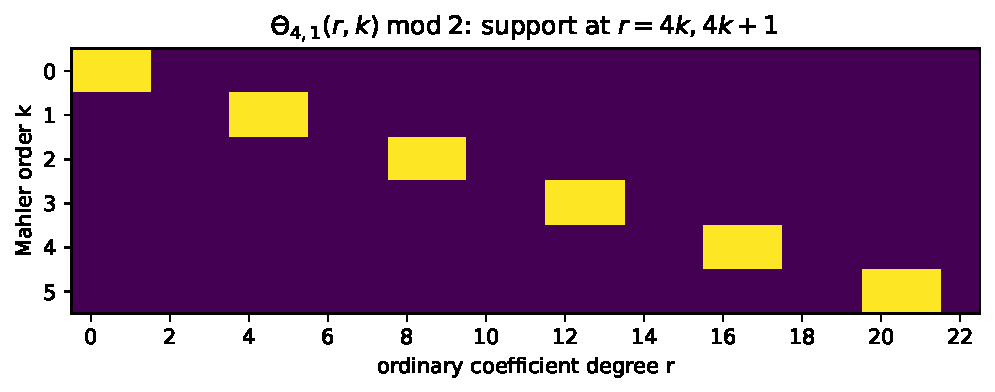
\includegraphics[width=.95\linewidth,height=3.15in,keepaspectratio]{../../figures/reconstructed/mahler_polyphase_kernel.pdf}
\caption{New reconstruction. The affine Mahler kernel has finite triangular support. At prime power radix its reduction is confined to a short Frobenius window.}
\label{hist:fig:mahler_polyphase_kernel}
\end{figure}

\subsubsection{Precision amplification}

\begin{histtheorem}[Scalar polyphase precision amplification]\label{hist:thm:scalar_polyphase_precision}
Let \(u\in\mathbb Z_p^\times\), let \(a,r\geq0\), and put
\[
H_a=
\begin{cases}
(p-1)p^a,&p\text{ odd},\\
2^{a+1},&p=2.
\end{cases}
\]
Then
\[
\boxed{
\Delta_{H_a}^{\,r}u^n
=
u^n\left(u^{H_a}-1\right)^r.
}
\]
For odd \(p\),
\[
\boxed{
\vp\left(\Delta_{H_a}^{\,r}u^n\right)
\geq(a+1)r.
}
\]
For \(p=2\) and odd \(u\),
\[
\boxed{
\vTwo\left(\Delta_{H_a}^{\,r}u^n\right)
\geq(a+3)r.
}
\]
Equivalently, every additional prime power digit increases the certified Mahler slope by one.
\end{histtheorem}

\begin{proof}
One difference with step \(H_a\) multiplies the unit mode by \(u^{H_a}-1\). Iterate. The valuation estimates are those of \cref{hist:cor:basic_local_difference_gains}.
\end{proof}

\begin{histlemma}[Matrix power amplification]\label{hist:lem:matrix_power_amplification}
\par\noindent\textbf{Editorial hypothesis correction.} Require $L\ge1$. At $L=0$ the standalone claim is false: for $p=3$, $d=1$ and $X=2=1+B$, one has $X^3-1=7\notin3\Z_3$. With $L\ge1$, every higher binomial term in the retained proof has the required valuation, including $p=2$.\par\medskip
If
\[
X=I+p^LB
\]
with \(B\in M_d(\Zp)\), then for every \(a\geq0\) there is \(B_a\in M_d(\Zp)\) such that
\[
\boxed{X^{p^a}=I+p^{L+a}B_a.}
\]
\end{histlemma}

\begin{proof}
Induct on \(a\). Expand the \(p\)th power of \(I+p^{L+a}B_a\). The linear term has valuation at least \(L+a+1\), and every higher term has at least that valuation.
\end{proof}

\begin{histtheorem}[Matrix polyphase precision amplification]\label{hist:thm:matrix_polyphase_precision}
\par\noindent\textbf{Editorial hypothesis correction.} Require $L\ge1$, $C,B\in M_d(\Z_p)$, $v_0,w\in\Z_p^d$, $H>0$, and $a,j,n,r\in\N$. These are the hypotheses of the two corrected matrix statements used by the retained proof. Without integral observation vectors or positive $L$, the preceding counterexamples invalidate the claimed precision.\par\medskip
Assume
\[
C^H=I+p^LB.
\]
Put \(H_a=Hp^a\). Then
\[
C^{H_a}=I+p^{L+a}B_a
\]
for an integral matrix \(B_a\). Every refined packet
\[
b_{a,j}(x)=a_{H_ax+j}
\]
has Mahler coefficients satisfying
\[
\boxed{\vp(c_{a,j,r})\geq(L+a)r.}
\]
Equivalently,
\[
\boxed{
\Delta_{H_a}^{\,r}a_n
\equiv0
\pmod {p^{(L+a)r}}.
}
\]
\end{histtheorem}

\begin{proof}
Combine \cref{hist:lem:matrix_power_amplification,hist:thm:matrix_carmichael_mahler}.
\end{proof}

\begin{histexample}[Refined dyadic Fibonacci ladder]\label{hist:ex:refined_fibonacci_ladder}
For the Fibonacci companion matrix
\[
C=
\begin{pmatrix}
1&1\\
1&0
\end{pmatrix},
\]
one has
\[
C^{12}
=I+8
\begin{pmatrix}
29&18\\
18&11
\end{pmatrix}.
\]
Therefore
\[
\boxed{
\Delta_{12\cdot2^a}^{\,r}F_n
\equiv0
\pmod {2^{(a+3)r}}.
}
\]
Every dyadic refinement doubles the step and adds one guaranteed binary digit at each Mahler depth.
\end{histexample}

\begin{figure}[t]
\centering
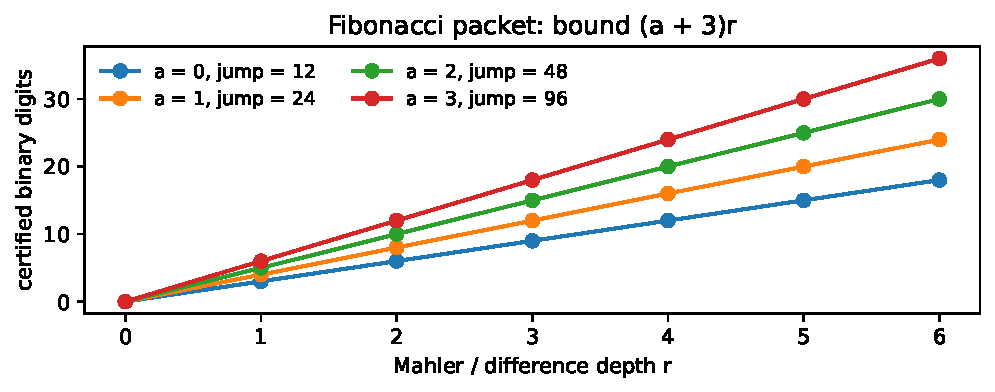
\includegraphics[width=.95\linewidth,height=3.15in,keepaspectratio]{../../figures/reconstructed/polyphase_precision_tree.pdf}
\caption{New reconstruction. Every additional prime power refinement digit increases the certified Mahler slope of a principal unit matrix packet by one.}
\label{hist:fig:polyphase_precision_tree}
\end{figure}

\subsubsection{Character and polyphase coordinates}

For odd \(p\), write
\[
\boxed{
n=j+(p-1)(s+p^aq),
}
\]
with \(0\leq j<p-1\) and \(0\leq s<p^a\). The address \(j\) records the finite character. The address \(s\) records the principal unit digit. The variable \(q\) carries the remaining Mahler expansion.

At the dyadic prime, write
\[
\boxed{
n=j+2(s+2^aq),
}
\]
with \(j\in\{0,1\}\) and \(0\leq s<2^a\). The sign coordinate replaces the odd prime character coordinate.

\begin{histproposition}[Local phase lattice]\label{hist:prop:local_phase_lattice}
For a unit mode \(u^n\), the odd prime coordinate gives
\[
\boxed{
u^n
=
u^{j+(p-1)s}
\left(u^{(p-1)p^a}\right)^q.
}
\]
The dyadic coordinate gives
\[
\boxed{
u^n
=
u^{j+2s}
\left(u^{2^{a+1}}\right)^q.
}
\]
Thus finite character phase, local digit address, and Mahler depth are separate coordinates.
\end{histproposition}

\begin{proof}
Substitute the two displayed decompositions of \(n\).
\end{proof}

\begin{histcorollary}[Polyphase refinement of the Euler branches]\label{hist:cor:euler_polyphase_refinement}
The analytic branches in \cref{hist:thm:odd_analytic_branch,hist:thm:direct_dyadic_interpolation} admit exact refinements under \(x=p^aq+s\). Their refined Mahler coefficients are obtained from \(\Theta_{p^a,s}\). The original monotone valuation ladders are preserved, and unit mode or invertible matrix representations gain one certified digit per refinement level.
\end{histcorollary}

\begin{proof}
Apply \cref{hist:thm:mahler_polyphase_transfer,hist:thm:polyphase_valuation_ledger,hist:cor:basic_local_difference_gains,hist:thm:matrix_polyphase_precision}.
\end{proof}

\begin{histremark}\label{hist:rem:polyphase_boundary}
Exact refinement does not imply that every branch is simpler. A simplification theorem requires an additional invariant, such as Frobenius sparsity, valuation gain, spectral collision, or a vanishing transfer block.
\end{histremark}
\subsection{Arithmetic lift obstructions}\label{hist:sec:lifting}

A congruence class may solve an equation to one precision and fail at the next. The correct obstruction is not an arbitrary residual vector. It is the residual vector modulo the image of the declared correction map.

\subsubsection{Linear lifting}

Let \(p\) be a prime. Let
\[
M\in M_{r,d}(\Zp),
\qquad
b\in\Zp^r.
\]
Suppose that \(x_L\in\Zp^d\) satisfies
\[
Mx_L\equiv b\pmod {p^L}
\]
for some \(L\geq1\). Define the reduced residual
\[
\rho_L(x_L)
=
\frac{Mx_L-b}{p^L}
\pmod p
\in\FF_p^r.
\]
Write \(\overline M\) for the reduction of \(M\) modulo \(p\).

\begin{histdefinition}[Linear lift obstruction]\label{hist:def:linear_lift_obstruction}
The linear obstruction at depth \(L\) is
\[
\boxed{
\operatorname{Ob}^{\mathrm{lin}}_L(x_L)
=
[\rho_L(x_L)]
\in
\coker(\overline M).
}
\]
\end{histdefinition}

\begin{histtheorem}[One level linear lifting]\label{hist:thm:linear_lifting}
A class represented by \(x_L\) lifts to a solution modulo \(p^{L+1}\) if and only if
\[
\boxed{
\operatorname{Ob}^{\mathrm{lin}}_L(x_L)=0.
}
\]
More precisely, a correction \(y\in\FF_p^d\) gives a lift
\[
x_{L+1}=x_L+p^Ly
\pmod {p^{L+1}}
\]
if and only if
\[
\boxed{
\overline My=-\rho_L(x_L).
}
\]
When one correction exists, the set of all correction classes is a coset of \(\ker\overline M\).
\end{histtheorem}

\begin{proof}
Modulo \(p^{L+1}\),
\[
M(x_L+p^Ly)-b
=
Mx_L-b+p^LMy.
\]
After division by \(p^L\) and reduction modulo \(p\), the lift condition becomes
\[
\rho_L(x_L)+\overline My=0.
\]
This equation is solvable exactly when the residual lies in the image of \(\overline M\). If \(y_0\) is one solution, every solution is \(y_0+z\) with \(z\in\ker\overline M\).
\end{proof}

\begin{histproposition}[Representative independence]\label{hist:prop:linear_obstruction_independence}
The class \(\operatorname{Ob}^{\mathrm{lin}}_L(x_L)\) depends only on the solution class of \(x_L\) modulo \(p^L\).
\end{histproposition}

\begin{proof}
Replace \(x_L\) by \(x_L+p^Lz\). The reduced residual changes by \(\overline Mz\). Its class in the cokernel is unchanged.
\end{proof}

\begin{histcorollary}[Exact number of linear children]\label{hist:cor:linear_child_count}
If \(\rho=\rank_{\FF_p}\overline M\), then a solvable depth \(L\) class has exactly
\[
\boxed{
p^{d-\rho}
}
\]
children modulo \(p^{L+1}\).
\end{histcorollary}

\begin{proof}
The correction set is a coset of a vector space of dimension \(d-\rho\).
\end{proof}

\begin{histexample}[A visible linear obstruction]\label{hist:ex:linear_lift_obstruction}
Take \(p=3\), \(L=1\), and
\[
M=
\begin{pmatrix}
1&1\\
0&0
\end{pmatrix}.
\]
The class \(x_1=(0,0)\) solves
\[
Mx_1\equiv b\pmod3
\]
for both
\[
b_1=(-3,0)
\qquad\text{and}\qquad
b_2=(0,-3).
\]
For \(b_1\), the reduced residual is \((1,0)\), which belongs to the image of \(\overline M\). There are three correction classes, given by
\[
y_1+y_2=2
\pmod3.
\]
For \(b_2\), the residual is \((0,1)\), whose cokernel class is nonzero. No lift modulo nine exists because the second row of \(M\) remains zero.
\end{histexample}

\begin{figure}[t]
\centering
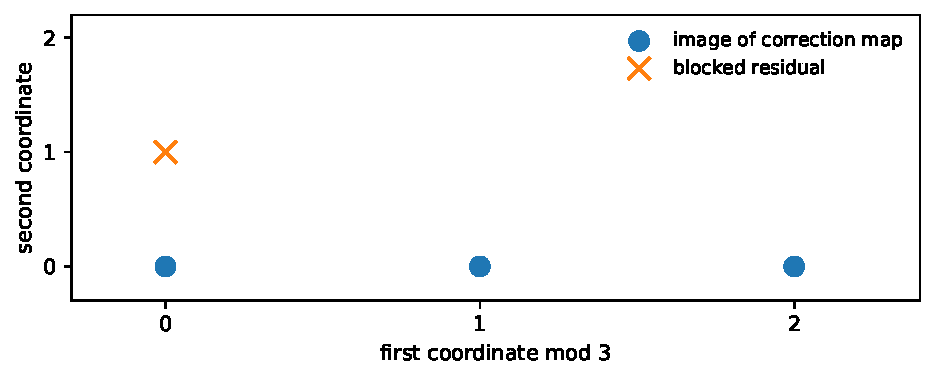
\includegraphics[width=.95\linewidth,height=3.15in,keepaspectratio]{../../figures/reconstructed/lift_obstruction.pdf}
\caption{New reconstruction. A residual vector lifts precisely when its class vanishes in the cokernel of the reduced correction map.}
\label{hist:fig:lift_obstruction}
\end{figure}

\subsubsection{Polynomial lifting}

Let
\[
F=(F_1,\ldots,F_r):\Zp^d\longrightarrow\Zp^r
\]
be a polynomial map.\par\noindent\textbf{Editorial coefficient clarification.} Here polynomial means $F_i\in\Z_p[X_1,\ldots,X_d]$, not merely an integer-valued polynomial with coefficients in $\Q_p$. This makes the Jacobian and Taylor remainder integral and their reduction well typed.\par Suppose
\[
F(x_L)\in p^L\Zp^r.
\]
Define
\[
\rho_L^F(x_L)
=
\frac{F(x_L)}{p^L}
\pmod p.
\]
Let \(J_F(x_L)\) denote the Jacobian matrix and write \(\overline J_F(x_L)\) for its reduction modulo \(p\).

\begin{histdefinition}[Polynomial lift obstruction]\label{hist:def:polynomial_lift_obstruction}
The polynomial obstruction at depth \(L\) is
\[
\boxed{
\operatorname{Ob}^{F}_L(x_L)
=
[\rho_L^F(x_L)]
\in
\coker\bigl(\overline J_F(x_L)\bigr).
}
\]
\end{histdefinition}

\begin{histtheorem}[One level polynomial lifting]\label{hist:thm:polynomial_lifting}
Let \(L\geq1\). A class represented by \(x_L\) lifts to a zero of \(F\) modulo \(p^{L+1}\) if and only if
\[
\boxed{
\operatorname{Ob}^{F}_L(x_L)=0.
}
\]
A correction \(y\in\FF_p^d\) gives a lift if and only if
\[
\boxed{
\overline J_F(x_L)y
=
-\rho_L^F(x_L).
}
\]
When a correction exists, the correction classes form a coset of
\[
\ker\overline J_F(x_L).
\]
\end{histtheorem}

\begin{proof}
The polynomial Taylor expansion gives
\[
F(x_L+p^Ly)
\equiv
F(x_L)+p^LJ_F(x_L)y
\pmod {p^{L+1}}.
\]
Every term of degree at least two in the increment contains \(p^{2L}\), which is divisible by \(p^{L+1}\). Divide by \(p^L\), reduce modulo \(p\), and apply the same cokernel criterion as in \cref{hist:thm:linear_lifting}.
\end{proof}

\begin{histproposition}[Polynomial representative independence]\label{hist:prop:polynomial_obstruction_independence}
The class \(\operatorname{Ob}^{F}_L(x_L)\) depends only on the class of \(x_L\) modulo \(p^L\).
\end{histproposition}

\begin{proof}
If \(x_L\) is replaced by \(x_L+p^Lz\), Taylor expansion shows that the reduced residual changes by an element of the image of \(\overline J_F(x_L)\). The reduced Jacobian itself is unchanged because \(L\geq1\).
\end{proof}

\begin{histcorollary}[Simple root lifting]\label{hist:cor:simple_root_lifting}
Assume \(r=d\) and
\[
\det J_F(x_L)\not\equiv0\pmod p.
\]
Then the depth \(L\) solution has exactly one child modulo \(p^{L+1}\). Iterating gives a unique \(p\) adic zero above the initial class.
\end{histcorollary}

\begin{proof}
The reduced Jacobian is invertible, so every residual has one correction. The resulting compatible sequence is Cauchy in \(\Zp^d\), and continuity of \(F\) gives a zero in the limit. Uniqueness holds at every depth.
\end{proof}

\begin{histexample}[A singular polynomial obstruction]\label{hist:ex:singular_polynomial_obstruction}
Let \(p=3\) and consider the class \(x_1=0\) modulo three. For
\[
F_0(x)=x^2,
\]
the residual and the reduced derivative both vanish. Every correction \(y\in\FF_3\) gives
\[
F_0(3y)\equiv0\pmod9,
\]
so the class has three children. For
\[
F_1(x)=x^2+3,
\]
the reduced derivative is still zero, but the reduced residual is one. Its class in the cokernel is nonzero, so no lift modulo nine exists.
\end{histexample}

This is the usual simple root mechanism behind Hensel lifting. The obstruction formulation also covers singular Jacobians, where some residual classes lift and others do not \cite{Serre1979,Gouvea1997,Robert2000}.

\subsubsection{Packetwise obstruction splitting}

\begin{histtheorem}[Packet decomposition of a lift obstruction]\label{hist:thm:packet_lift_obstruction}
Suppose
\[
\FF_p^d
=
\bigoplus_{a\in A}U_a,
\qquad
\FF_p^r
=
\bigoplus_{a\in A}V_a,
\]
and suppose a linear correction map \(D:\FF_p^d\to\FF_p^r\) satisfies
\[
D(U_a)\subseteq V_a
\]
for every \(a\). Write \(D_a=D|_{U_a}\). Then
\[
\boxed{
\coker D
\cong
\bigoplus_{a\in A}\coker D_a.
}
\]
A residual lifts if and only if every packet obstruction vanishes.
\end{histtheorem}

\begin{proof}
The image of \(D\) is the direct sum of the images of the maps \(D_a\). Taking the quotient of the codomain packet decomposition gives the stated cokernel decomposition.
\end{proof}

\begin{histremark}\label{hist:rem:lifting_boundary}
The obstruction theorems solve one declared local lifting step. They do not prove that a compatible branch exists across unrelated primes, that a global Diophantine point exists, or that an arithmetic representation is automorphic.
\end{histremark}

\subsection{Recurrence packets and a common integral spine}\label{hist:sec:recurrences}

Linear recurrences provide a setting where residue subsequences, local completions, and a common global source can all be described exactly. Background on recurrence sequences may be found in \cite{EverestVanDerPoortenShparlinskiWard2003,Stanley2012}.

\subsubsection{Companion jumps}

Let \(R\) be a commutative ring. Let
\[
v_{n+1}=Cv_n,
\qquad
C\in M_d(R).
\]
For a positive integer \(N\) and an address \(j\in\{0,\ldots,N-1\}\), define the residue state packet
\[
u_k^{(j)}=v_{Nk+j}.
\]

\begin{histtheorem}[Companion jump recurrence]\label{hist:thm:companion_jump}
Every residue state packet satisfies
\[
\boxed{
u_{k+1}^{(j)}=C^Nu_k^{(j)}.}
\]
More explicitly,
\[
\boxed{
u_k^{(j)}=C^j(C^N)^kv_0.}
\]
\end{histtheorem}

\begin{proof}
The state relation gives \(v_n=C^nv_0\). Substitute \(n=Nk+j\).
\end{proof}

\begin{figure}[t]
\centering
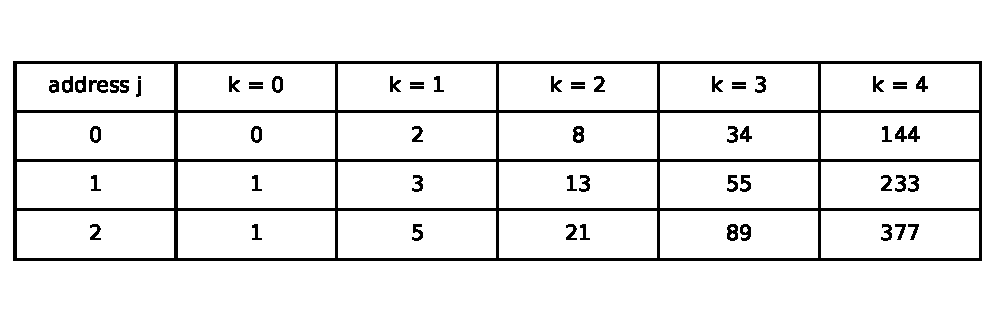
\includegraphics[width=.95\linewidth,height=3.15in,keepaspectratio]{../../figures/reconstructed/recurrence_packets.pdf}
\caption{New reconstruction. Fibonacci residues $F_{3k+j}$, with $F_0=0$ and $F_1=1$. Each packet evolves by the same jump matrix \(C^3\) and has a different initial address.}
\label{hist:fig:recurrence_packets}
\end{figure}

We use the resultant convention
\[
\Res_y(f,g)
=
\prod_{f(\alpha)=0}g(\alpha)
\]
when \(f\) is monic, with roots counted with multiplicity.

\begin{histtheorem}[Characteristic polynomial of the jump]\label{hist:thm:jump_characteristic}
Let
\[
\chi_C(y)=\det(yI-C).
\]
Then
\[
\boxed{
\chi_{C^N}(x)
=
\Res_y\bigl(\chi_C(y),x-y^N\bigr).
}
\]
The identity holds over the coefficient ring after interpreting the resultant universally.
\end{histtheorem}

\begin{proof}
After passage to an algebraic closure, let \(\alpha_1,\ldots,\alpha_d\) be the eigenvalues of \(C\), counted with algebraic multiplicity. The resultant is
\[
\prod_{i=1}^{d}(x-\alpha_i^N),
\]
which is the characteristic polynomial of \(C^N\). Both sides are polynomial expressions with integer coefficients in the entries of \(C\), so the identity descends to every commutative coefficient ring.
\end{proof}

\begin{figure}[t]
\centering
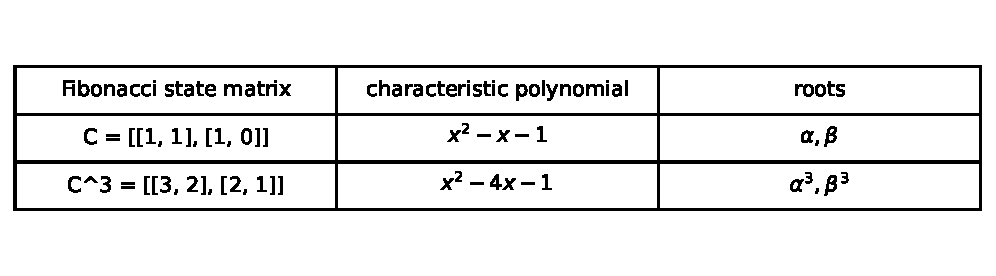
\includegraphics[width=.95\linewidth,height=3.15in,keepaspectratio]{../../figures/reconstructed/recurrence_root_power.pdf}
\caption{New reconstruction. Passing to every \(N\)th term raises each characteristic root to its \(N\)th power.}
\label{hist:fig:recurrence_root_power}
\end{figure}

\subsubsection{Second order recurrences}

\begin{histtheorem}[Residue subsequences of a second order recurrence]\label{hist:thm:second_order_jump}
Suppose
\[
x_{n+2}=Px_{n+1}-Qx_n
\]
over a commutative ring. Define \(V_0=2\), \(V_1=P\), and
\[
V_{n+2}=PV_{n+1}-QV_n.
\]
For every positive integer \(N\) and every address \(j\), the subsequence
\[
u_k=x_{Nk+j}
\]
satisfies
\[
\boxed{
u_{k+2}=V_Nu_{k+1}-Q^Nu_k.}
\]
\end{histtheorem}

\begin{proof}
The companion matrix
\[
C=
\begin{pmatrix}
P&-Q\\
1&0
\end{pmatrix}
\]
has trace \(P\) and determinant \(Q\). The trace of \(C^N\) is \(V_N\), while its determinant is \(Q^N\). Cayley Hamilton applied to \(C^N\) gives
\[
(C^N)^2-V_NC^N+Q^NI=0.
\]
Apply this identity to the residue state packet and take its scalar coordinate.
\end{proof}

\begin{histcorollary}[Fibonacci residue packets]\label{hist:cor:fibonacci_packets}
Let \(F_0=0\), \(F_1=1\), and \(F_{n+2}=F_{n+1}+F_n\). Let \(L_N\) denote the Lucas number. For every \(N\geq1\) and every address \(j\),
\[
\boxed{
F_{N(k+2)+j}
=
L_NF_{N(k+1)+j}
-(-1)^NF_{Nk+j}.
}
\]
\end{histcorollary}

\begin{proof}
Apply \cref{hist:thm:second_order_jump} with \(P=1\) and \(Q=-1\). Then \(V_N=L_N\).
\end{proof}

\subsubsection{Finite and local periodicity}

\begin{histtheorem}[Periodicity of an invertible recurrence modulo a prime power]\label{hist:thm:recurrence_periodicity}
Let
\[
C\in M_d(\ZZ),
\qquad
p\nmid\det C.
\]
For every \(L\geq1\), every state orbit modulo \(p^L\) is purely periodic. Its period divides the order of \(C\) in
\[
\operatorname{GL}_d(\ZZ/p^L\ZZ).
\]
If \(p\mid\det C\), every orbit is still eventually periodic.
\end{histtheorem}

\begin{proof}
When \(p\nmid\det C\), multiplication by \(C\) is a permutation of the finite state set \((\ZZ/p^L\ZZ)^d\). Every orbit of a permutation is periodic, and applying the group order relation for \(C\) gives the divisibility statement. Without invertibility, repeated application of a map on a finite set eventually repeats a state, after which the orbit is periodic.
\end{proof}

\begin{histcorollary}[Residue packet periods]\label{hist:cor:residue_packet_periods}
Under the invertibility hypothesis of \cref{hist:thm:recurrence_periodicity}, every residue packet with jump \(N\) has period dividing the order of \(C^N\) modulo \(p^L\).
\end{histcorollary}

\begin{proof}
Use the jump matrix from \cref{hist:thm:companion_jump}.
\end{proof}

\subsubsection{The common integral spine}

\begin{histtheorem}[Base change of an integral recurrence]\label{hist:thm:integral_recurrence_spine}
Let
\[
C\in M_d(\ZZ),
\qquad
v_0\in\ZZ^d.
\]
The integral orbit
\[
v_n=C^nv_0
\]
determines, by base change, compatible orbits in every ring \(R\) equipped with a homomorphism \(\ZZ\to R\). In particular, the reductions modulo every positive integer and the orbits in every \(\Zp^d\) share the same companion matrix, characteristic polynomial, and integer recurrence relations.
\end{histtheorem}

\begin{proof}
Every coordinate of \(C^nv_0\) is an integer polynomial in the entries of \(C\) and \(v_0\). Applying a ring homomorphism commutes with matrix multiplication and preserves every polynomial relation with integer coefficients.
\end{proof}

\begin{histcorollary}[Prime independent recurrence spine]\label{hist:cor:prime_independent_spine}
An integral companion system gives a canonical common source for all of its local realizations. No choice of coefficient prime is required to define the recurrence or its residue packets.
\end{histcorollary}

\begin{proof}
Apply \cref{hist:thm:integral_recurrence_spine} to the companion matrix and its initial state.
\end{proof}

\begin{histremark}\label{hist:rem:spine_boundary}
This theorem supplies a prime independent spine for integral linear recurrences. It does not prove that every unrelated family of local arithmetic packets arises from one global object.
\end{histremark}

\subsection{Chinese remainder packet refinement}\label{hist:sec:crt}

The Chinese remainder theorem gives an exact factorization of residue addresses. We state it at the level of sequence projectors so that it can be combined directly with the earlier coordinate systems.

\begin{histdefinition}[Residue projector]\label{hist:def:residue_projector}
For a sequence \(a=(a_n)_{n\geq0}\), a positive integer \(N\), and an address \(r\) modulo \(N\), define
\[
(P_{N,r}a)_n
=
\begin{cases}
a_n,&n\equiv r\pmod N,\\
0,&n\not\equiv r\pmod N.
\end{cases}
\]
\end{histdefinition}

\begin{histproposition}[Complete residue packet system]\label{hist:prop:residue_packet_system}
For fixed \(N\), the projectors \(P_{N,r}\) satisfy
\[
P_{N,r}P_{N,s}
=
\delta_{rs}P_{N,r}
\]
and
\[
\boxed{
\sum_{r\bmod N}P_{N,r}=I.
}
\]
\end{histproposition}

\begin{proof}
Every nonnegative integer belongs to exactly one residue class modulo \(N\).
\end{proof}

\begin{histtheorem}[Coprime packet factorization]\label{hist:thm:crt_packet_factorization}
Let \(A\) and \(B\) be coprime positive integers. Let \(r_A\) be an address modulo \(A\) and \(r_B\) an address modulo \(B\). Let \(r\) be the unique address modulo \(AB\) satisfying
\[
r\equiv r_A\pmod A,
\qquad
r\equiv r_B\pmod B.
\]
Then
\[
\boxed{
P_{AB,r}
=
P_{A,r_A}P_{B,r_B}
=
P_{B,r_B}P_{A,r_A}.
}
\]
\end{histtheorem}

\begin{proof}
The product retains exactly the indices satisfying both congruences. By the Chinese remainder theorem, those indices form one residue class modulo \(AB\) \cite{IrelandRosen1990}.
\end{proof}

\begin{histcorollary}[Several coprime moduli]\label{hist:cor:many_crt_packets}
Let \(N_1,\ldots,N_s\) be pairwise coprime and put
\[
N=\prod_{j=1}^{s}N_j.
\]
For compatible addresses \(r_j\),
\[
\boxed{
P_{N,r}
=
\prod_{j=1}^{s}P_{N_j,r_j},
}
\]
where \(r\) is the unique combined address modulo \(N\).
\end{histcorollary}

\begin{proof}
Iterate \cref{hist:thm:crt_packet_factorization}.
\end{proof}

\begin{figure}[t]
\centering
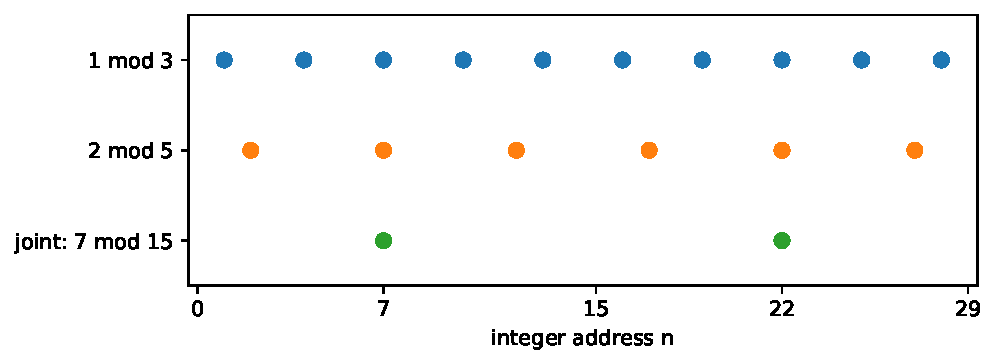
\includegraphics[width=.95\linewidth,height=3.15in,keepaspectratio]{../../figures/reconstructed/crt_packets.pdf}
\caption{New reconstruction. A residue modulo a product of coprime moduli is the exact intersection of its local residue packets.}
\label{hist:fig:crt_packets}
\end{figure}

\begin{histstandardfact}[Finite local reconstruction]\label{hist:fact:finite_local_reconstruction}
Let
\[
N=\prod_{j=1}^{s}p_j^{a_j}
\]
be the prime power factorization of a positive integer. The map
\[
\ZZ/N\ZZ
\longrightarrow
\prod_{j=1}^{s}\ZZ/p_j^{a_j}\ZZ
\]
is a ring isomorphism. Thus a compatible collection of prime power residues reconstructs one residue modulo \(N\) \cite{IrelandRosen1990}.
\end{histstandardfact}

\begin{histproposition}[Dyadic and odd residue refinement]\label{hist:prop:dyadic_odd_refinement}
Let \(N=2^am\) with \(m\) odd. Every residue packet modulo \(N\) factors uniquely as the product of one dyadic packet modulo \(2^a\) and one odd packet modulo \(m\).
\end{histproposition}

\begin{proof}
The moduli \(2^a\) and \(m\) are coprime. Apply \cref{hist:thm:crt_packet_factorization}.
\end{proof}

\begin{histremark}\label{hist:rem:crt_weight_boundary}
The residue address factors exactly, but valuation weights do not become identical across primes. The odd coordinate system of \cref{hist:sec:local_euler} and the dyadic coordinate system of \cref{hist:sec:local_euler} remain genuinely different integral charts.
\end{histremark}

\subsection{Verification and exact boundaries}\label{hist:sec:boundaries}

The proofs in the article are symbolic. Exact computation tests formulas, finite ranges, and the source implementation. It does not replace a uniform proof.

\begin{table}[t]
\centering
\caption{Status of the principal local arithmetic blocks.}
\label{hist:tab:status}
\begin{tabular}{>{\raggedright\arraybackslash}p{.33\textwidth}>{\raggedright\arraybackslash}p{.24\textwidth}>{\raggedright\arraybackslash}p{.31\textwidth}}
\toprule
Block & Status & Main boundary\\
\midrule
Standard window period & Proved modulo the residue prime & Higher prime powers require inverse estimates\\
Unified local Euler transfer & Proved for every prime & Odd and dyadic integral charts remain different\\
Dyadic kernel and truncation & Exact weight and optimal uniform modulus proved & Row cancellation may give stronger values\\
Carmichael and Mahler transfer & Proved for scalar, polynomial exponential, matrix, and finite adelic systems & A jump congruence must first be available\\
Local Euler interpolation & Proved for depleted odd branches and the direct dyadic branch & The odd nonunit factor is only evaluated at integer interpolation points\\
Affine polyphase transfer & Exact analysis, synthesis, carry law, kernel composition, residual sparsity, and valuation preservation proved & General exact kernel valuations remain open\\
Lift obstruction and recurrence spine & Proved for the declared local problems and integral recurrences & Unrestricted global gluing is not proved\\
\bottomrule
\end{tabular}
\end{table}

\subsubsection{The remaining congruential difference problem}

Let \(C_{mp,j}(n)\) be a congruential reciprocal coefficient and let
\[
h=\frac{p-1}{m}.
\]
The unit mode calculations suggest bounds for
\[
\vp\left(\Delta_h^sC_{mp,j}(n)\right).
\]
The theorems of \cref{hist:sec:mahler,hist:sec:polyphase} determine the gain before the congruential triangular inverse is applied. They do not yet determine every valuation loss introduced by that inverse. The full family bound therefore remains open.

\subsubsection{Higher valuations of the affine kernel}

The residual formula
\[
\Theta_{p^a,s}(r,k)
\equiv
\binom{s}{r-p^ak}
\pmod p
\]
is exact. A closed formula for
\[
\vp\left(\Theta_{p^a,s}(r,k)\right)
\]
in terms of base \(p\) carries and the three digit addresses is not proved here. Such a formula would sharpen the min plus valuation ledger and could distinguish optimal refinement trees.

\subsubsection{The remaining global gluing problem}

The finite adelic theorem synchronizes a finite set of primes when one integral state system is already fixed. The recurrence theorem gives a common local source under the same assumption. Chinese remainder projectors reconstruct finite residue addresses. None of these results proves that an arbitrary collection of local analytic branches has a common global arithmetic origin.

\begin{figure}[t]
\centering
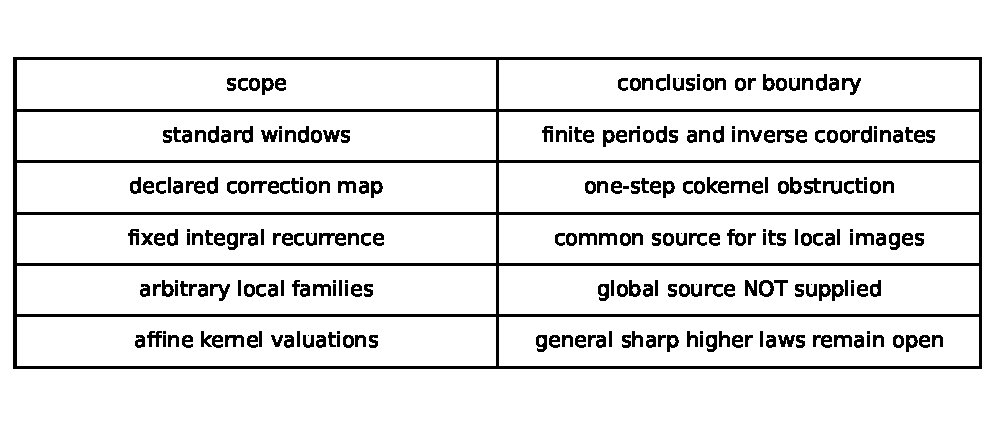
\includegraphics[width=.95\linewidth,height=3.15in,keepaspectratio]{../../figures/reconstructed/claim_boundary.pdf}
\caption{New reconstruction. The proved local coordinate theory and the remaining inverse valuation, affine kernel, and global gluing problems.}
\label{hist:fig:claim_boundary}
\end{figure}

\subsubsection{Historical scope}

The article uses classical work on Euler congruences, finite differences, local fields, Hurwitz series, Mahler interpolation, Lucas congruences, and recurrence sequences \cite{CarlitzLevine1960,Young1999,Young2001,Sun2008,Chen2004,Lucas1878a,LidlNiederreiter1997,EverestVanDerPoortenShparlinskiWard2003}. The exact formulas and local transfer statements should be compared individually with that literature before any historical priority claim is made.

\subsection{Conclusion}\label{hist:sec:conclusion}

The local arithmetic theory now has one common architecture. The finite character coordinate identifies the torsion phase. The source and kernel product reconstructs the Euler coefficient. The kernel valuation records certified precision. Carmichael and Mahler coordinates describe the remaining principal unit motion. Polyphase analysis resolves additional local digits, records carries and shifts exactly, and transports Mahler coefficients through a finite affine kernel.

The odd and dyadic cases agree at the level of convolution and differ at the level of integral geometry. At odd primes the source must be depleted before it becomes a unit mode interpolation. At the dyadic prime the source extends directly to an analytic integral function. The dyadic kernel has exact weight \(4r-1\), giving the optimal uniform modulus \(2^{4M+3}\) after depth \(M\).

Three tasks remain outside the proved region. The first is a complete finite difference estimate after the congruential triangular inverse. The second is an exact higher valuation theory for the affine Mahler kernel. The third is a global existence theorem for local systems that do not already arise from one integral source.

\par\smallskip\noindent\textbf{Current status.} This dated statement is superseded for the stated divisor-branch family by Theorem~\ref{thm:arith-divisor-base}, with the $j!$ normalization and factorial valuation loss explicitly retained. It makes no claim for unrestricted families.\par


